\chapter{$\Delta \rm F$=2}
\label{sec:DF2}

\section{Introduction} %% 2 
%%% mixing amplitudes
The meson-antimeson ocillations are described by the mixing amplitudes~\cite{Altmannshofer:2009ne}
\begin{equation}
M_{12}^{(M)} \equiv \left \langle M | \mathcal{H}_{\rm eff}^{\Delta F = 2} | \bar{M} \right \rangle \ \, M = K^0, B_{d,s}
\end{equation}
%%% hamiltonian 
Where $\mathcal{H}_{\rm eff}^{\Delta F = 2}$ is the \textit{effective} Jamiltonian. Within the MSSM, it has the form:
\begin{equation}
\mathcal{H}_{\rm eff}^{\Delta F = 2}  = \sum_{i=1}^{5}C_i Q_i + \sum_{i=1}^{3}\tilde{C}_i\tilde{Q}_i + \rm h.c.
\end{equation}
with the operators $Q_i$ given, in the case of $B_s$ mixing, by:
\begin{equation}
\begin{split}
& Q_1 = (\bar{s}^{\alpha}\gamma_{\mu}P_Lb^{\alpha})(\bar{s}^{\beta}\gamma^{\mu}P_Lb^{\beta}) \\
& Q_2 = (\bar{s}^{\alpha}P_Lb^{\alpha})(\bar{s}^{\beta}P_Lb^{\beta}) \\
& Q_3 = (\bar{s}^{\alpha}P_Lb^{\beta})(\bar{s}^{\beta}P_Lb^{\alpha}) \\
& Q_4 = (\bar{s}^{\alpha}P_Lb^{\alpha})(\bar{s}^{\beta}P_Rb^{\beta}) \\
& Q_5 = (\bar{s}^{\alpha}P_Lb^{\beta})(\bar{s}^{\beta}P_Rb^{\alpha})
\end{split}
\label{eq:WOBs}
\end{equation}
where $P_{R,L} = \frac{1}{2}(1 \pm \gamma_5)$ and $\alpha,\beta$ are colour indices. The operators $\tilde{Q}_{1,2,3}$ are obtained from $Q_{1,2,3}$ by the replacement $L \leftrightarrow R$~\cite{Altmannshofer:2009ne}. In the case of $B_d$, the replacement $s \rightarrow d$ needs to be done in equation \ref{eq:WOBs}. 
Several representative observables can be extracted from these ampliudes, such as the mixing phase, the oscillation frequency or the semileptonic asymmetry:
\begin{equation}
\phi_s = \arg{(M_{12})}, \ \Delta m_s = |M_{12}|, \ A_{SL} = -\frac{\Delta\Gamma_s}{\Delta M_s} \tan{\phi_s}
\end{equation}
Note that their value strongly depends on NP contributions:
\begin{equation}
M_{12} = M_{12}^{SM} + M_{12}^{NP} 
\end{equation}
The experimental search of the weak mixing angle is discussed in detail in \ref{sec:phisEXP}. Theoretical interpretations \red{of this result} are reviewed in \ref{sec:phisPHEN}, and a \texttt{MultiNest} scan~\cite{Feroz:2008xx} is presented in \ref{sec:phisMULT}. 

\section{$\phi_s$ experimental} %% 10
\label{sec:phisEXP}

In the SM, \textit{CP}-violation originates from a single-phase in the Cabibbo-Kobayashi-Maskawa (CKM) quark-mixing matrix~\cite{Charles:2011va}, as explained in \ref{sec:CKMMatrix}. There are 3 different kinds of \textit{CP}-violation for neutral mesons, \textit{e.g.} $B_s^0$ and $\bar{B}_s^0$:
\begin{enumerate}
\item Direct \textit{CP}-violation: originated by a difference in the amplitudes associated to the direct decay of the $B_s^0$ and $\bar{B_s^0}$ mesons into the same final state %% CP eigenstate final 
\item \textit{CP}-violation in the $B_s^0- \bar{B}_s^0$ oscillation, that arises when the oscillation from $B_s^0$ to $\bar{B}_s^0$ is different from the oscillation from $\bar{B}_s^0$ to $B_s^0$
\item \textit{CP}-violation in the interference between the amplitudes  associated to the direct decay of a $B_s^0$ meson into a \textit{CP}-eigenstate final state and those associated to the decay after $B_s^0- \bar{B}_s^0$ oscillation
\end{enumerate} 
This last type of \textit{CP}-violation is characterized by the \textit{CP}-violating phase, $\phi_s$, defined as:
\begin{equation}
 \label{eq:phis}
\phi_s^f = -\rm arg(\lambda_f),\ \lambda_f = \eta_f \frac{q}{p}\frac{\bar{\mathcal{A}}_f}{\mathcal{A}_f},
\end{equation}
where \textit{f} is the final state, $\eta_f$ is 1(-1) for CP-even(CP-odd) states, $\left| \frac{q}{p} \right |$ determines the amount of \textit{CP}-violation in mixing, and ${\mathcal{A}}_f$($\bar{\mathcal{A}}_f$) is the amplitude of the $B_s^0$($\bar{B}_s^0$) meson decaying into a given final state, \textit{f}.
Precision measurements of this phase are needed in order to properly disentagle SM and NP contributions.

 In the SM, for $b\to c\overline{c}s$ transitions and ignoring subleading penguin contributions, this phase is predicted to be $-2\beta_s$, where $\beta_s=\arg\left[
 - (V_{ts} V_{tb}^*) / (V_{cs} V_{cb}^*)\right]$ and $V_{ij}$ are elements of the CKM quark flavour mixing
 matrix~\cite{Kobayashi:1973fv,Cabibbo:1963yz}. The indirect determination via global fits to experimental data gives
 \mbox{$2\beta_s=0.0364\pm0.0016\rad$}\red{~\cite{Charles:2011va}}. This precise indirect determination within the SM makes the
 measurement of $\phi_s$ interesting since new physics (NP) processes could modify
 the phase if new particles were to contribute to the $B_s^0$--$\bar{B}_s^0$\ box diagrams~\cite{Buras:2009if,Chiang:2009ev}.
 
\begin{figure}[h]
	\begin{center}
		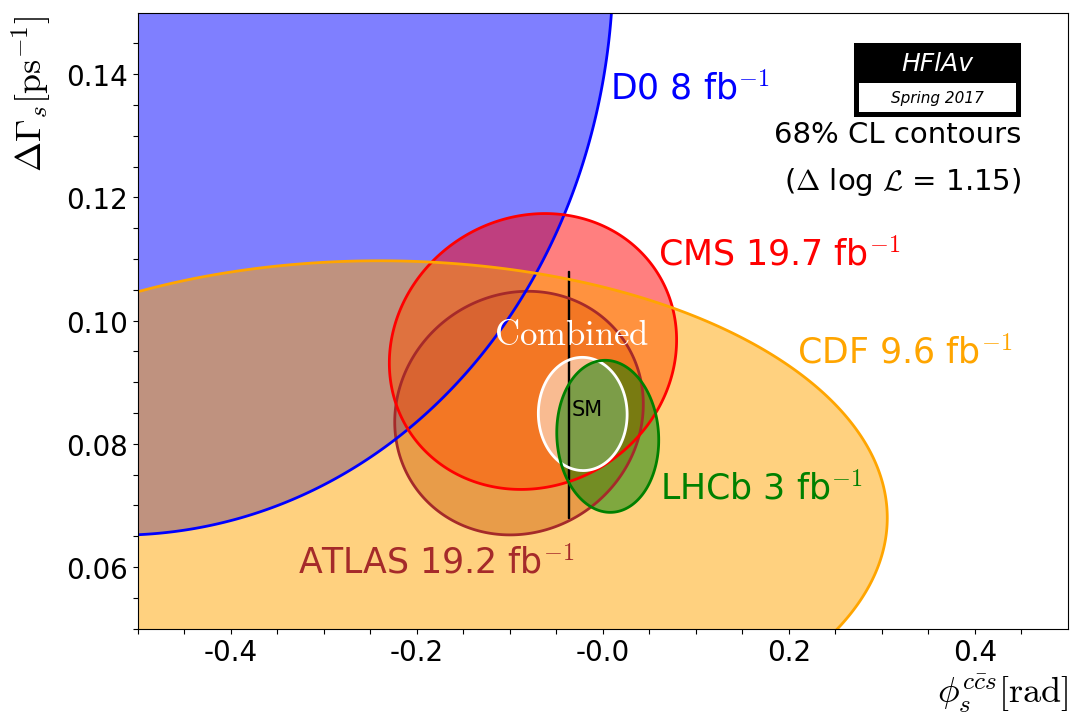
\includegraphics[width=0.5\linewidth]{figs/Spring2017_Phis_vs_DGs.png}
	\end{center}
	\caption{\label{fig:HFAG}\small
		Individual 68$\%$ confidence-level contours of ATLAS, CMS, CDF, D0 and LHCb in the $(\phi_s^{c\overline{c}s},\Delta \Gamma_s)$, their combined contour (solid line  and shaded area), as well as the SM predictions (thick black rectangle) as performed by the HFLAV \cite{HFLAV2017} averaging group.
	}
\end{figure} 
 
The situation after including all Run 1 results from LHCb, and all results from ATLAS, CMS, CDF and D0 is shown in Figure~\ref{fig:HFAG}.
Current preliminary world averages (and their correlations) for the $CP$ violating phase $\phi_s$ and the decay width difference in the $B^0_s$ system, $\Delta \Gamma_s$, are:
\begin{eqnarray*}
\phi_s = -0.021 \pm 0.031\,\mathrm{rad} \\
\Delta \Gamma_s = 0.085 \pm 0.006\, \mathrm{ps}^{-1}\\
\rho( \phi_s ,  \Delta \Gamma_s ) =  -0.0095
\end{eqnarray*}

The aim of this analysis is to perform the measurement of $\phi_s$ in the \mbox{$B_s^0 \rightarrow J/\psi K^+ K^-$} channel by
adding a further $2\invfb$ of integrated luminosity collected at $13\tev$ in Run 2 of LHC in 2015 and 2016.
In addition, updated measurements of the decay width difference of the light (L)
and heavy (H) $B_s^0$ mass eigenstates,
$\Delta\Gamma_s \equiv \Gamma_{\mathrm L} - \Gamma_{\mathrm H}$, and the ratio between the
average widths in the $B_s^0$ and in the $B_d^0$ systems, $\Gamma_s/\Gamma_d$. 

\subsection{Phenomenology}
The baseline fit is obtained assuming that direct $CP$ violation caused by penguin diagrams is the same for all polarization states, therefore $\lambda_f$ is considered to be independent of the polarization state, $f$. Checks were made to check this ansatz. 

The theoretical differential decay rate for an initial $B_s^0$ as a function of decay time and angles using polarization dependent $\lambda_f = |\lambda_f|e^{-i \phi_s^f} \equiv |\lambda_f|e^{-i \phi_f} $ ($f=0,\,{||},\,{\perp},\,{\rm S}$) is given as~\cite{Liu:2013nea}
\begin{eqnarray}
 \frac{d^4 \Gamma( t) }{dm_{KK }^2 d\cos\theta_K d\cos\theta_l d\phi}&=&  \sum_{k=1}^{10} N_k h_k(t) f_k(\theta_K, \theta_l, \phi),  \label{eq:rate_mult_lambda}
 \end{eqnarray}
where the decay-time-dependent functions $h_k(t)$ are given as
\begin{eqnarray}
 h_k(t)= \frac{3}{ 4\pi}
   e^{-\Gamma t}\left\{ a_k \cosh\frac{\Delta \Gamma t}{2} + b_k \sinh\frac{\Delta \Gamma t}{2} + c_k \cos(\Delta mt)  +  d_k \sin(\Delta mt) \right\}.
\label{eq:rate_mult_lambda2}
\end{eqnarray}
For an initial $\bar{B}_s^0$ at production, the signs of $c_k$ and $d_k$ should be reversed. \red{appendix with coefficients?}
For the purpose of reducing correlation between fit parameters, it can be chosen to fit for $|\lambda_0|$, $\phi_0$ and $|{{\lambda_f}\over {\lambda_0}}|$, $\phi_f-\phi_0$, for $f \neq 0$.

\subsection{Samples and event selection}

In this section, the data and simulated samples used in this analysis are introduced, together with the trigger, stripping and offline selections applied to these samples.

\subsubsection{Data sample}

The analysis presented in this report uses a data sample collected at the LHCb
experiment at the LHC\@. The dataset corresponded to a total integrated
luminosity $\int{\mathcal{L}}{1.9 \rm fb^{-1}}$. Of this, $0.3 \rm fb^{-1}$ were taken in 2015 at a centre-of-mass energy $\sqrt{s}$ = 13$\rm TeV$ and $1.6 \rm fb^{-1}$ were taken in 2016 at $\sqrt{s}$ = 13$\rm TeV$.

Stripping version 26 was used for 2016 data and stripping version 24 was
used for 2015 data.  All stripping versions use exactly the same selection,
based on the {\tt StrippingBetaSBs2JpsiPhiDetached} {\tt
StrippingBetaSBd2JpsiKstDetached} and {\tt StrippingBetaSBu2JpsiKDetached} lines
in the DIMUON stream.  The data samples were processed using {\tt DaVinci} version
v42r1 and momentum scaling has been applied.

\subsubsection{Simulation samples}

In the LHCb simulation, $pp$ collisions are generated using
{\tt Pythia} with a specific \lhcb\ configuration~\cite{Sjostrand:2006za,
LHCb-PROC-2010-056}.

\begin{table}[h]
\begin{center}
\begin{tabular}{lcccc}
    \hline
    Event type & Decay mode & Options & Year & Events \\
    \hline
    \multicolumn{5}{c}{Signal modes}\\
    \hline
    13144004 & $\Bs\to\jpsi\phi$ & {\tt Update2012,dG=0,DecProdCut,S26} &  2016 & 25M \\
    13144011 & $\Bs\to\jpsi\phi$ & {\tt Update2016,DecProdCut,S26} & 2016 & 20M \\
    13144011 & $\Bs\to\jpsi\phi$ & {\tt Update2012,DecProdCut,S28} & 2016 & 10M \\
    13144011 & $\Bs\to\jpsi\phi$ & {\tt Update2016,DecProdCut,S24} & 2015 & XXM \\
    13144041 & $\Bs\to\jpsi\Kp\Km$ & {\tt DecProdCut} & 2016 & 7M \\
    %13100004 & $\Bs\to\jpsi\Kp\Km$ & {\tt Higher s-waves,DecProdCut} & 2016 & 20M \\
    \hline
    \multicolumn{5}{c}{Backgrounds}\\
    \hline
    15144001 & $\Lb\to\jpsi p\Km$    & {\tt PHSP, DecProdCut} &  XXX & XXM \\
    24142001 & Inclusive Jpsi & {\tt JpsiInAcc} &  2016 & 20M \\
    \hline
    \multicolumn{5}{c}{Control samples}\\
    \hline
    11144001 & $B^0 \to J/\psi K^{*0}$    & {\tt Update2016,DecProdCut,S24} & 2015  & 10M \\
    11144001 & $B^0 \to J/\psi K^{*0}$    & {\tt Update2016,DecProdCut,S26} & 2016  & 10M \\
    12143001 & $B^+ \to J/\psi K^+$    & {\tt Update2016,DecProdCut,S24} & 2015  & 10M \\
    12143001 & $B^+ \to J/\psi K^+$    & {\tt Update2016,DecProdCut,S26} & 2016  & 10M \\
    24142001 & Inclusive Jpsi & {\tt JpsiInAcc} &  2016 & 20M \\
    \hline
    \multicolumn{5}{c}{Generator Level}\\
    \hline
\end{tabular}
\caption{MC samples used in the analysis. SXX indicates the stripping version that is used to flag the events. DecProdCut means that all the daughters are required to be within LHCb acceptance.
}
\label{tab:mc}
\end{center}
\end{table}

Decays of hadronic particles are described by {\tt EvtGen}~\cite{Lange:2001uf}, in which final state radiation is generated using {\tt Photos}~\cite{Golonka:2005pn}. The {\tt Geant4} toolkit simulates the interaction of the generated particles with the detector, and the detector
response~\cite{Agostinelli:2002hh, Allison:2006ve}. Further details of the
simulation process can be found in Ref.~\cite{LHCb-PROC-2011-006}. The simulated data is processed in a very similar way to the real data, with the stripping run in flagging mode,
with no prescales applied for the trigger. Sim09b was used for the simulated samples.  The samples used are listed in Table~\ref{tab:mc}.

Simulated signal samples are used to determine the angular acceptance.  As will be discussed in Sec.~\ref{subsec:AngAcc}, the samples are reweighted to match various distributions observed in data before obtaining the final acceptance.  Similarly, the $\Lambda^0_b$ and the $B^0$ samples are used for background studies and decay time acceptance studies, respectively.  This is discussed in Sec.~\ref{subsec:MassFit} and Sec.~\ref{subsec:TimeAcc}, respectively.
The $B^+$ sample is used for tagging studies as described in Sec.~\ref{subsec:Tagging}.

The main physics parameters used in the main simulation used in this analysis, \texttt{Eventtype = 13144011, Bs\_Jpsiphi,mm=CPV,update2016,DecProdCut}, are summarized in Table~\ref{tab:evtgendecaypars13144011}. For simulated samples a momentum smearing is applied in order to reproduce better the distributions in data.

\begin{table}[h]
 \caption{\small Decay model parameters for the Sim09b MC sample used in this analysis, \texttt{Eventtype = 13144011, Bs\_Jpsiphi,mm=CPV,update2016,DecProdCut}.}
 \centerline{
   \begin{tabular}{cc}
      Parameter &       Value\\
     \hline
     $\Delta m_s$            & 17.8\invps \\
     $\Delta\Gamma_s$        & 0.08543\invps \\
     $\Gamma_s$              & 0.6614\invps \\
     $\phis$               & $-0.03$\rad  \\
     $|A_0(0)|^2$            & 0.5242 \\
     $|A_\|(0)|^2  $         & 0.2256  \\
     $|A_\perp(0)|^2  $       & 0.2500   \\
     $\delta_\|-\delta_0 $   & 3.26\rad  \\
     $\delta_\perp-\delta_0 $ & 3.08\rad \\\hline
   \end{tabular}}
 \label{tab:evtgendecaypars13144011}
\end{table}

\subsubsection{Stripping selection}

In order to select  $\Bs\to\jpsi\phi$ events, in data and MC we start from the stripping line {\tt StrippingBetaSBs2JpsiPhiDetachedLine}, whose selection can be found in Table \ref{tab:Bs2Jpsiphistripping}.
We use {\tt Stripping version 26} or {\tt 28} for 2016 and {\tt Stripping version 24} for 2015. In both cases the selection is the same.\\

 \renewcommand{\arraystretch}{1.2}
\begin{table}[h]
  \centering
  \caption{Selection criteria used to identify $B^0_s \to J/\psi \phi$ candidates.}
    \begin{tabular}{lrcc}\hline\hline
            &  Variable                        & Stripping \\
      \hline
      all tracks                       & $\chi^2_{\rm track}/{\rm nDoF}$                                & $<3$                     \\
       \hline
       $J/\psi \to \mu^{+} \mu^{-}$      &  $\Delta \mathrm{ln} \mathcal{L}_{{\mu}{\pi}}$ ($\mu^{\pm}$)   & $>0$                      \\
 			               &  $p_{T}$   ($\mu^{\pm}$)                                      & $>500\,\rm MeV/c$             \\
                                       & $\chi^2_{\rm DOCA}$                                           & $ < 20$                    \\
                                       & $\chi^2_{\rm vtx}/{\rm nDoF}$                                 & $ < 16$                    \\
               		               & $m(\mu^+\mu^-)$                                              &  $\in [3020,\,3170]\rm MeV/c^2$ \\
      \hline
      $\phi \to K^+ K^-$                & $\chi^2_{\rm DOCA}$                                           & $ < 30$                    \\
                                       &  $p_{T}$ ($\phi$)                                             & $>500\,\rm MeV/c$              \\
		                       & $m(K^+K^-)$                                                & $\in [980,\,1050]\rm MeV/c^2$                \\
                                       & $\chi^2_{\rm vtx}/{\rm nDoF}$                                 & $ < 25$                    \\
                                       & $\Delta \mathrm{ln} \mathcal{L}_{{K}{\pi}}$ $(K^+)$           & $>0$                          \\
      \hline
      $B^0_s \to \Jpsi \phi$           & $m(\jpsi\Kp\Km)$                                           & $\in [5150,\,5550]\mathrm{MeV/c^2}$  \\
                                       & $\chi^2_{\rm vtx}/{\rm nDoF}$                                 &  $< 20$  \\
                                       & $t$                                                          & $>0.2$ ps               \\
      \hline
    \end{tabular}
\label{tab:Bs2Jpsiphistripping}
\end{table}
\renewcommand{\arraystretch}{1.0}

For time resolution studies we use the stripping line {\tt BetaSBs2JpsiPhiPrescaledLine}, which has the same selection as shown in Table~\ref{tab:Bs2Jpsiphistripping} apart from the cut on the decay time of the $B^0_s$ candidate.

\subsubsection{Trigger selection}
\label{sec:trigger}

The following trigger strategy has been identified in order to retain the largest number of signal events while keeping a small number of trigger lines.
\begin{itemize}
\item No L0 requirements
\item HLT1 selection: {\tt Jpsi\_Hlt1DiMuonHighMassDecision\_TOS} or {\tt B\_Hlt1TrackMuonDecision\_TOS} or {\tt B\_Hlt1TwoTrackMVADecision\_TOS}
\item HLT2 selection: {\tt Jpsi\_Hlt2DiMuonDetachedJPsiDecision\_TOS}
\end{itemize}

\subsubsection{Corrections}
Corrections are applied to the simulated samples to match the distributions obtained from data:

\begin{enumerate}
        \item The stripped and triggered $B_s^0 \to J/\psi K^+K^-$ candidates are taken, with the $B_s^0$ decay time restricted to the range [0.3,15] ps. 
	\item The data invariant mass distribution of stripped and triggered $B_s^0 \to J/\psi K^+K^-$  candidates is fitted to obtain an sWeighted sample of data that is used in the following steps.
        %\item For MC, on top of the selection mentioned before only background categories 0 (signal), 50 (radiative events) with true decay time different from 0 and 60 (ghosts) are included (see Appendix~\ref{Appendix_BKGCAT} for a more detailed explanation).
        \item For MC, on top of the selection mentioned before only background categories 0 (signal) and 50 (radiative events) with true decay time different from 0 are included %%\red{more details?}.
	\item The simulation PID variable distributions are corrected using the {\tt PIDCalib} package.
	\item Using the above data sample, the $B_s^0$ production kinematics, nTracks distribution and the muon/kaon track ghost probability variables are reweighted.
\end{enumerate}

A BDT is trained to further improve the signal to background ratio. It is trained with 2016 samples. Namely, the 2016 corrected simulated sample for the signal sample while 2016 data candidates with $5450\rm MeV/c^2 < m(J/\psi K^+ K^-) < 5550\rm MeV/c^2$ are used
for the background sample.
Special care was taken to avoid variables that could introduce angular or decay time efficiencies, like impact parameter $\chi^2$ of final
state particles, the direction angle of the $B^0_s$ (DIRA) or transverse momentum of final state particles.
The figure of merit used to optimise the BDT response is given by
\begin{equation}
	{\rm FOM} = \frac{(\sum_i w_i)^2}{\sum_i w_i^2},
\end{equation}
where the index $i$ runs over all candidates in the sample and  $w_i$ are
per-candidate weights that are determined from the invariant mass fit
that is performed at each point in the scan over the BDT response. Figure~\ref{fig:FOM} shows on the left how the figure of merit performs and on the right the number of signal events divided by its uncertainty, both as a function of the BDT response. A similar distribution is observed. The optimal value is found to be at $> 0.78$.
After the BDT requirement has been applied there are
approximately 102\,000 signal candidates and 26\,000 background candidates
in the mass window of the fit, $5320\rm MeV/c^2 < m(J/\psi K^+ K^-) < 5420\rm MeV/c^2$ in 2016. The signal to background ratio is $\sim 3.9$. 
The mass fit used to determine sweights to statistically
remove this background and also the removal of peaking backgrounds for both 2015 and 2016 data samples is described in detail in the next \red{section}.

\begin{figure}[t]
	\begin{center}
    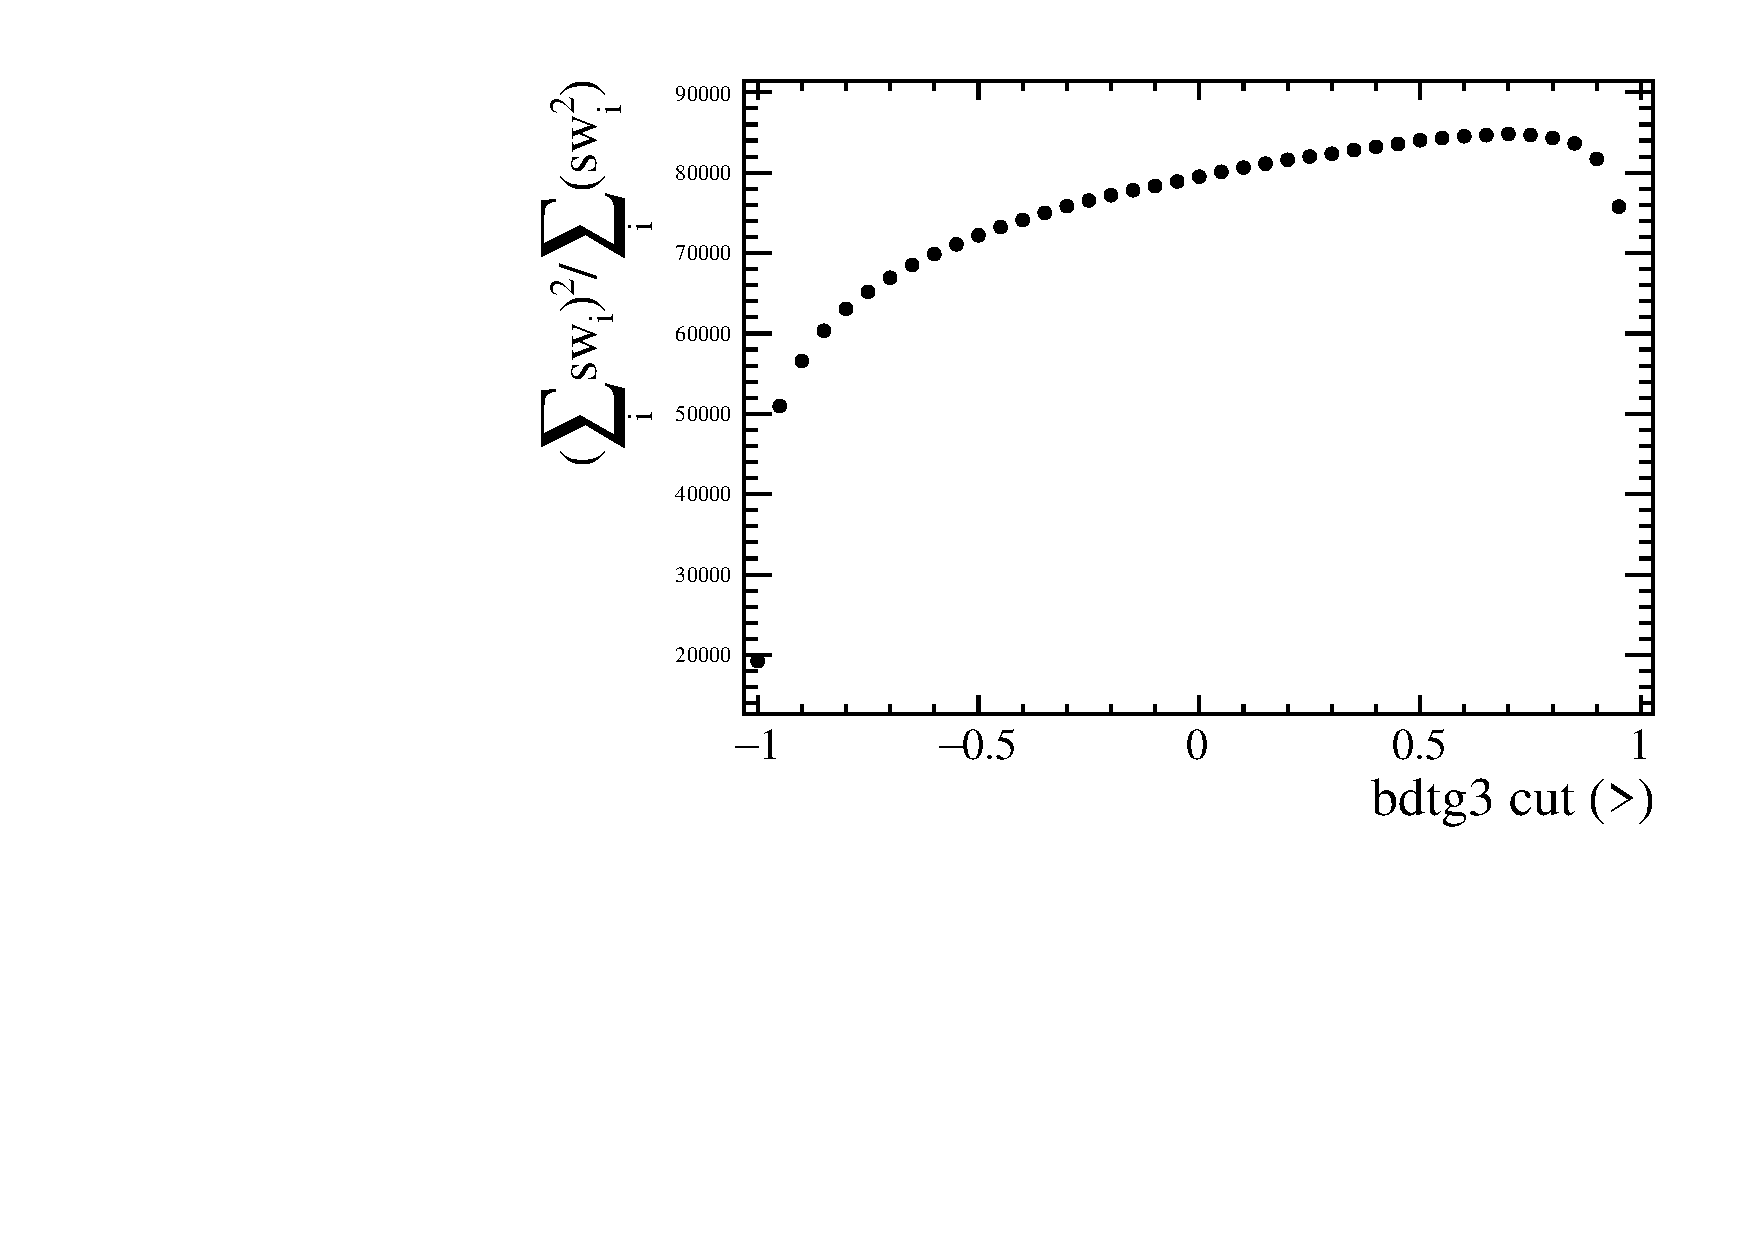
\includegraphics[width=0.49\linewidth]{figs/bs_2016_FOM}
		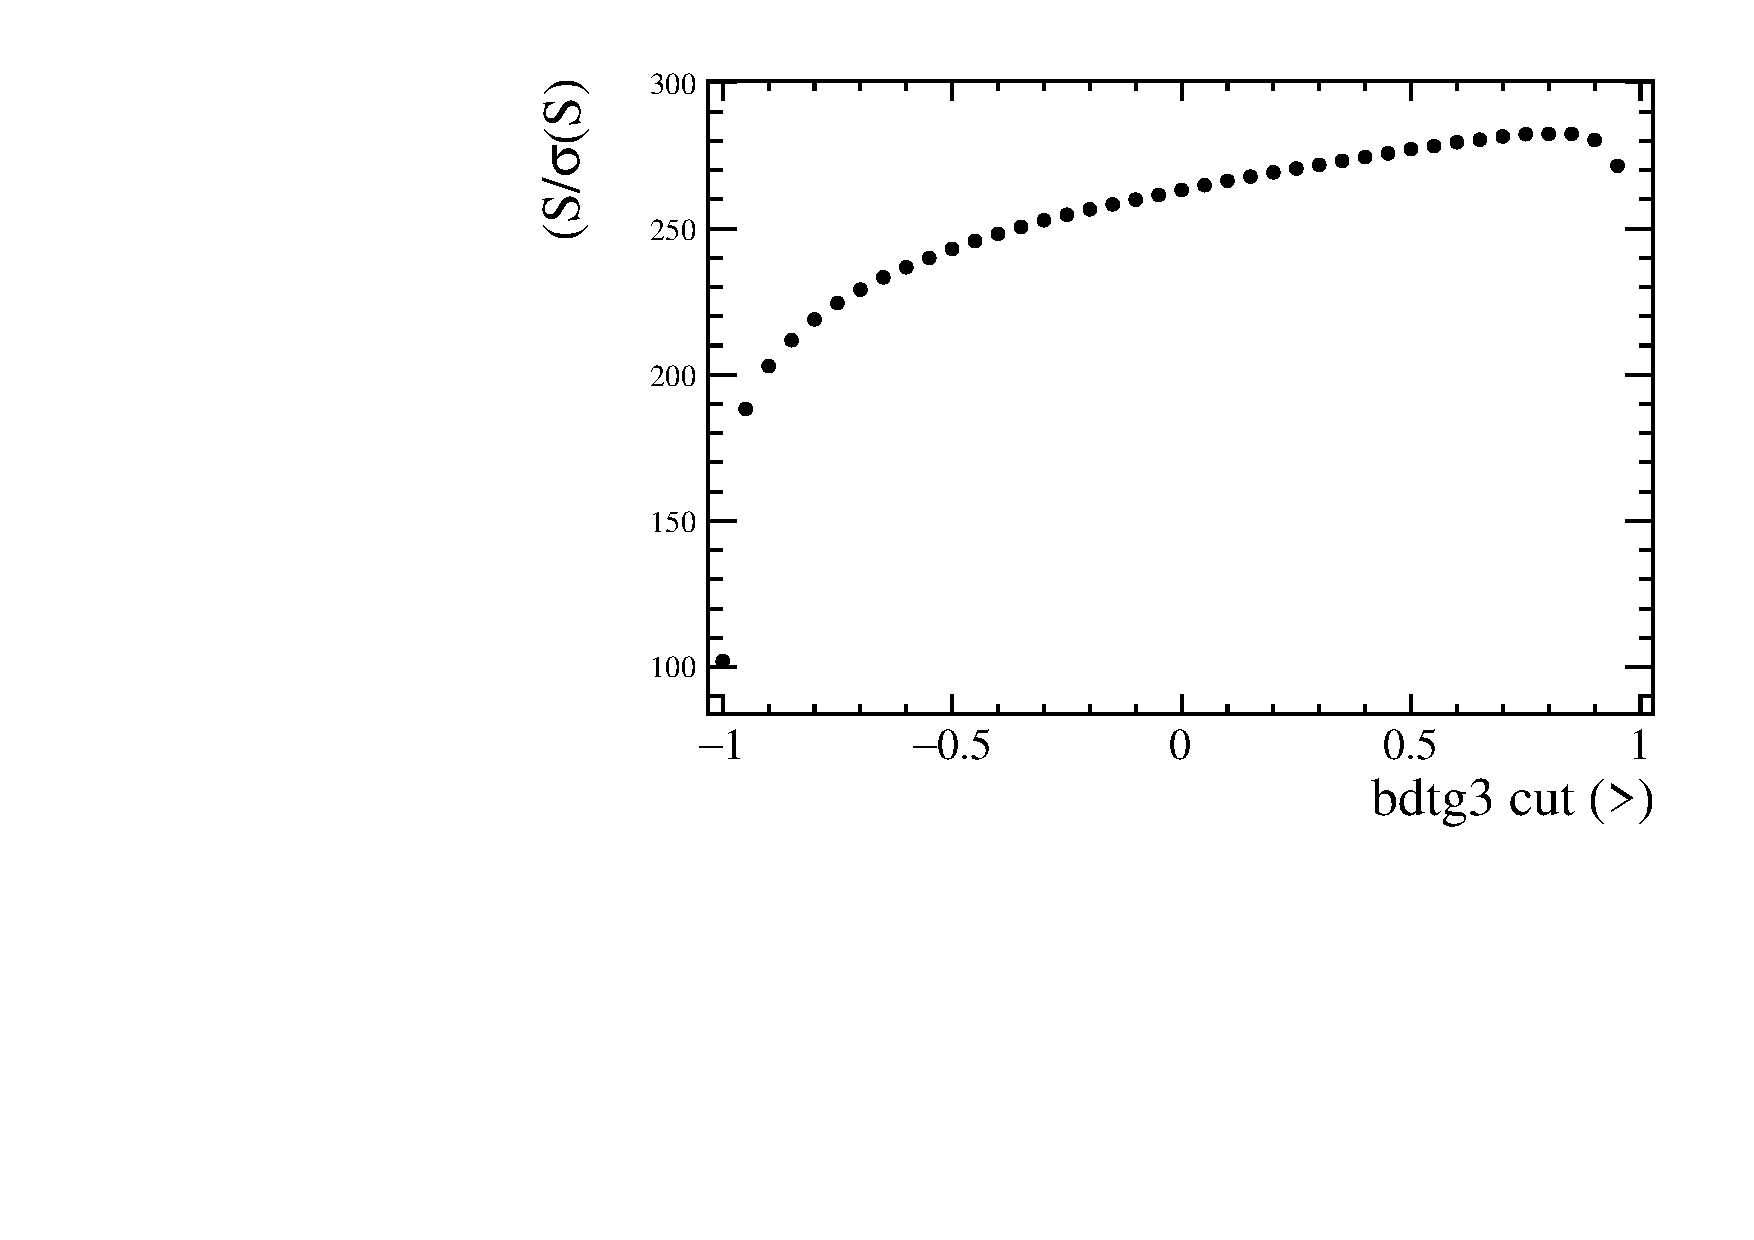
\includegraphics[width=0.49\linewidth]{figs/bs_2016_S_SIGMAS}
	\end{center}
	\caption{\label{fig:FOM}\small
		Distribution of the figure of merit used to optimise the cut on the BDT response (left) and distribution of signal yield divided by its uncertainty (right).}
\end{figure}

\subsection{Mass fit and computation of signal sWeights}
\label{subsec:MassFit}
The physics parameter of interest are extracted via a log-likelihood fit of the signal PDF to the unbinned decay time and anguar distributions. The events are first weighted to statistically subtract the background components using the \textit{sPlot} method~\cite{sWeights} with $m(J/\psi K^+ K^-)$ as the discriminating variable. 

In order to have an improved resolution, the $m(J/\psi K^+ K^-)$ is determined using both the $J/\psi$ mass and PV constraints. The combinatorial background is modelled with an exponential function and the signal distribution with a double-sided \textit{Crystal Ball} (CB) function. The double-sided CB function uses the per-event mass error as conditional observable, so that the correlation between $\cos{\theta_{\mu}}$ and mass resolution is taken into account. The full \textit{p.d.f} is the following: 

\begin{align*}
p &= N_{sig} CB(x;\mu,\alpha_1,\alpha_2,n_1,n_2,s_1,s_2 | \sigma_{i}) \\
&+ N_{bkg}((1-f_{B_d})e^{-\gamma_b x} + f_{B_d} Gauss(x;\mu_{B_d},\sigma_{B_d}),
\end{align*}
where $N_{sig}$ and $N_{bkg}$ is a number of signal and background events
correspondingly, $\mu$ is the mean of the distribution,
$s_1$ and $s_2$ are the scale factors, which accounts for underestimation of the per-event
mass error, $\alpha_1, \alpha_2, n_1, n_2$ are the tail parameters,
$\gamma_b$ is the coefficient in the exponential to describe the background.

The background sources that are considered consist in:
\begin{itemize}
\item $B^0 \rightarrow J/\psi K^{*0}$ peaking background, vetoed using PID cuts. 
\item $\Lambda_b^0 \rightarrow J/\psi pK^-$ peaking background, vetoed using PID cuts. The remaining events are statistically subtracted by injecting simulated events into the data tupe with a negative sum of weights equal to the expected number of events. 
\item $B^0 \rightarrow J/\psi K^+ K^-$ peaking background, modelled with a Gaussian in the nominal mass fit. 
\end{itemize}

For the fit to the $m(J/\psi K^+ K^-)$ distribution, the sample is divided
into twenty-four subsamples, each with an independent signal fraction and different
signal mass shapes. The subsamples correspond to six bins in the $K^+K^-$ mass,
namely [990, 1008, 1016, 1020, 1024, 1032, 1050] MeV/$c^2$, two trigger 
categories:
\begin{itemize}
\item \textbf{``Biased"}: {\tt B\_Hlt1TrackMuonDecision\_TOS} or {\tt B\_Hlt1TwoTrackMVADecision\_TOS} and not {\tt Jpsi\_Hlt1DiMuonHighMassDecision\_TOS} 
\item \textbf{``Unbiased"}: {\tt Jpsi\_Hlt1DiMuonHighMassDecision\_TOS}
\end{itemize}
and two years of the data-taking~(2015 and 2016). 

The event multipliciy (ratio between the number of events containing more than one cndidate and the total number of events) is found to be 1.2\% in the full $B_s^0$ mass region, but only 0.2\% for candidates in the signal region. Most of these candidates 
are due to cases where the $J/\psi$ is shared and one or two different kaons are added, making these events truly combinatorial in character. Given the low fraction of multiple events, it is evaluated as a systematic contribution removed them randomly. 

\subsection{\texorpdfstring{$C_{\rm SP}$}{Csp} factors}
\label{sec:CSP}
%LHCb-INT-2012-017
The relative change of the S-wave $m_{KK}$ line shape with respect to that of the P wave has to be considered in the interference terms of the angular expressions, as we are
performing the analysis in finite $m_{KK}$ bins (see Ref.~\cite{xie_CSP_sfiterror} for a detailed discussion). This is taken into account by adding a multiplicative correction factor, $C_{\rm SP}$, to the signal PDF, namely to the S-P-wave interference terms with $k=8,9,10$ in Eq. \eqref{eq:rate_mult_lambda}, i.e. $N_{k}\rightarrow C_{{\rm SP},i} N_{k}$. There are in total six  $C_{\rm SP}$ factors, one for each $m_{KK}$ bin.

The line shapes of the P and S wave are denoted as $p(m_{KK})$ and $s(m_{KK})$, respectively, where both are normalised to unity over a range $[m_{KK}^L,m_{KK}^U]$.
Essentially, the issue is that $\langle p\times s^*\rangle \neq \langle p \rangle \times \langle s^*\rangle$ in each $m_{KK}$ bin. Therefore, the product $p \times s^*$ is integrated, as it appears in the interference terms between the P and S wave. This yields

\begin{equation}
\label{eq:CSP}
\frac{\int_{m_{KK}^L}^{m_{KK}^H} { p \times s^*}  \:\:d m_{KK}}
{\sqrt{\int_{m_{KK}^L}^{m_{KK}^H} { |p|^2}  \:\:d m_{KK} \int_{m_{KK}^L}^{m_{KK}^H} { |s|^2}  \:\:d m_{KK}}}
 = C_{\rm SP} e^{-i \theta_{\rm SP}},
\end{equation}
where $C_{\rm SP}$ is the correction factor and the phase $\theta_{\rm SP}$ is
absorbed in the measurement of  $\delta_{\rm S} - \delta _{\perp}$.%phase space
model The shape of the P wave is a Breit-Wigner distribution, the same as in
Eq.(4) of Ref.~\cite{Liu:2241242}. The S-wave line shape is an $f_{0}$ with pole
mass of $0.9499$ GeV$/c^{2}$ as measured in Ref.~\cite{Liu:2241242}. Both the
$f_0$ and $\phi$ resonance distributions include a phase space factor $ \left (
\sqrt{\frac{P_B}{m_B}\frac{P_R}{\sqrt{s_{23}}}} \right )$, two Blatt-Weisskopf
factors for the \B and the $\Kp\Km$ resonance, and birth and decay momenta of
the $f_0, \phi$ and $\Bs$, where $L_B = 1, L_R = 0$ for $f_0$ and $L_B = 0, L_R
= 1$ for $\phi$. Note that the $f_0$ mass is considered to be 949 \mev. This
value, different from the PDG one ($990 \pm 30$ \mev)~\cite{PDG2017}, is taken
from the $\Bs\to\jpsi\pi^+\pi^-$ measurement~\cite{Aaij:2014emv}.

The detector reolution effect on the $C_{\rm SP}$ factors needs to be taken into account. While Eq.\ref{eq:CSP} is defined in dependence on the true $m_{KK}$, the mass bins are defined in dependence on the measured $m_{KK}$. The resolution effect can be incorporated as an efficiency correction, $\epsilon_i(m_{KK})$, of the $C_{\rm SP}$ factors
according to  
\begin{equation}
C_{SP} e^{-i \theta_{SP}} = \frac{\int_{2m_K}^{m_{B_s^0}-m_{J/\psi}} { p \times s^*\times \epsilon(m_{KK})}  \:\:d m_{KK}}{\sqrt{\int_{2m_K}^{m_{B_s^0}-m_{J/\psi}} { |p|^2\times \epsilon(m_{KK})} 
\:\:d m_{KK} \int_{2m_K}^{m_{B_s^0}-m_{J/\psi}} { |s|^2\times \epsilon(m_{KK})}  \:\:d m_{KK}}},
\label{eq:Csp2}
\end{equation}
\noindent where $\epsilon(m_{KK})$ is
\begin{equation}
\epsilon(m_{KK}) =
\begin{cases}
1, \text{ if $m_L< m_{KK} < m_H$} \\
0 \text{ otherwise}.
\end{cases},
\end{equation}
in the case where we bin in the true $m_{KK}$ mass (or equivalently, have perfect resolution). In reality though, we cut on a measured mass that has a finite resolution, and hence $\epsilon_{i}(m_{KK})$ will have a non-trivial structure. Note that in this definition we should consider events in the true $m_{KK}$ spectrum up to $2.27$ GeV/$c^{2}$, 
which is the value of $m_{B_s^0}-m_{J/\psi}$. However, the $\phi$ contribution after a certain point in $m_{KK}$ is too small to be modelled well in MC, so we apply an upper limit cut at $1.06$ GeV/$c^{2}$.
We use simulated events from the 2016 MC sample with and without S wave (see \tabref{tab:mc}) to determine $\epsilon_i(m_{KK})$ by dividing the $m_{KK}$ histogram before and after the selection of the events in each bin.
\figref{fig:epsilon_m} shows the corresponding distributions. We use the $C_{\rm SP}$ obtained from the MC without S wave with exception of the first bin, where the MC with S wave is used. The reason for this is that
in the region of $m_{KK}$, the contribution of the S wave is the largest and the MC with S wave has more events. With this, we obtain the $C_{\rm SP}$ factors shown in \tabref{tab:CSP1}.

\begin{figure}
\begin{center}
% \includegraphics[width=1.\textwidth]{figs/epsilon.pdf}
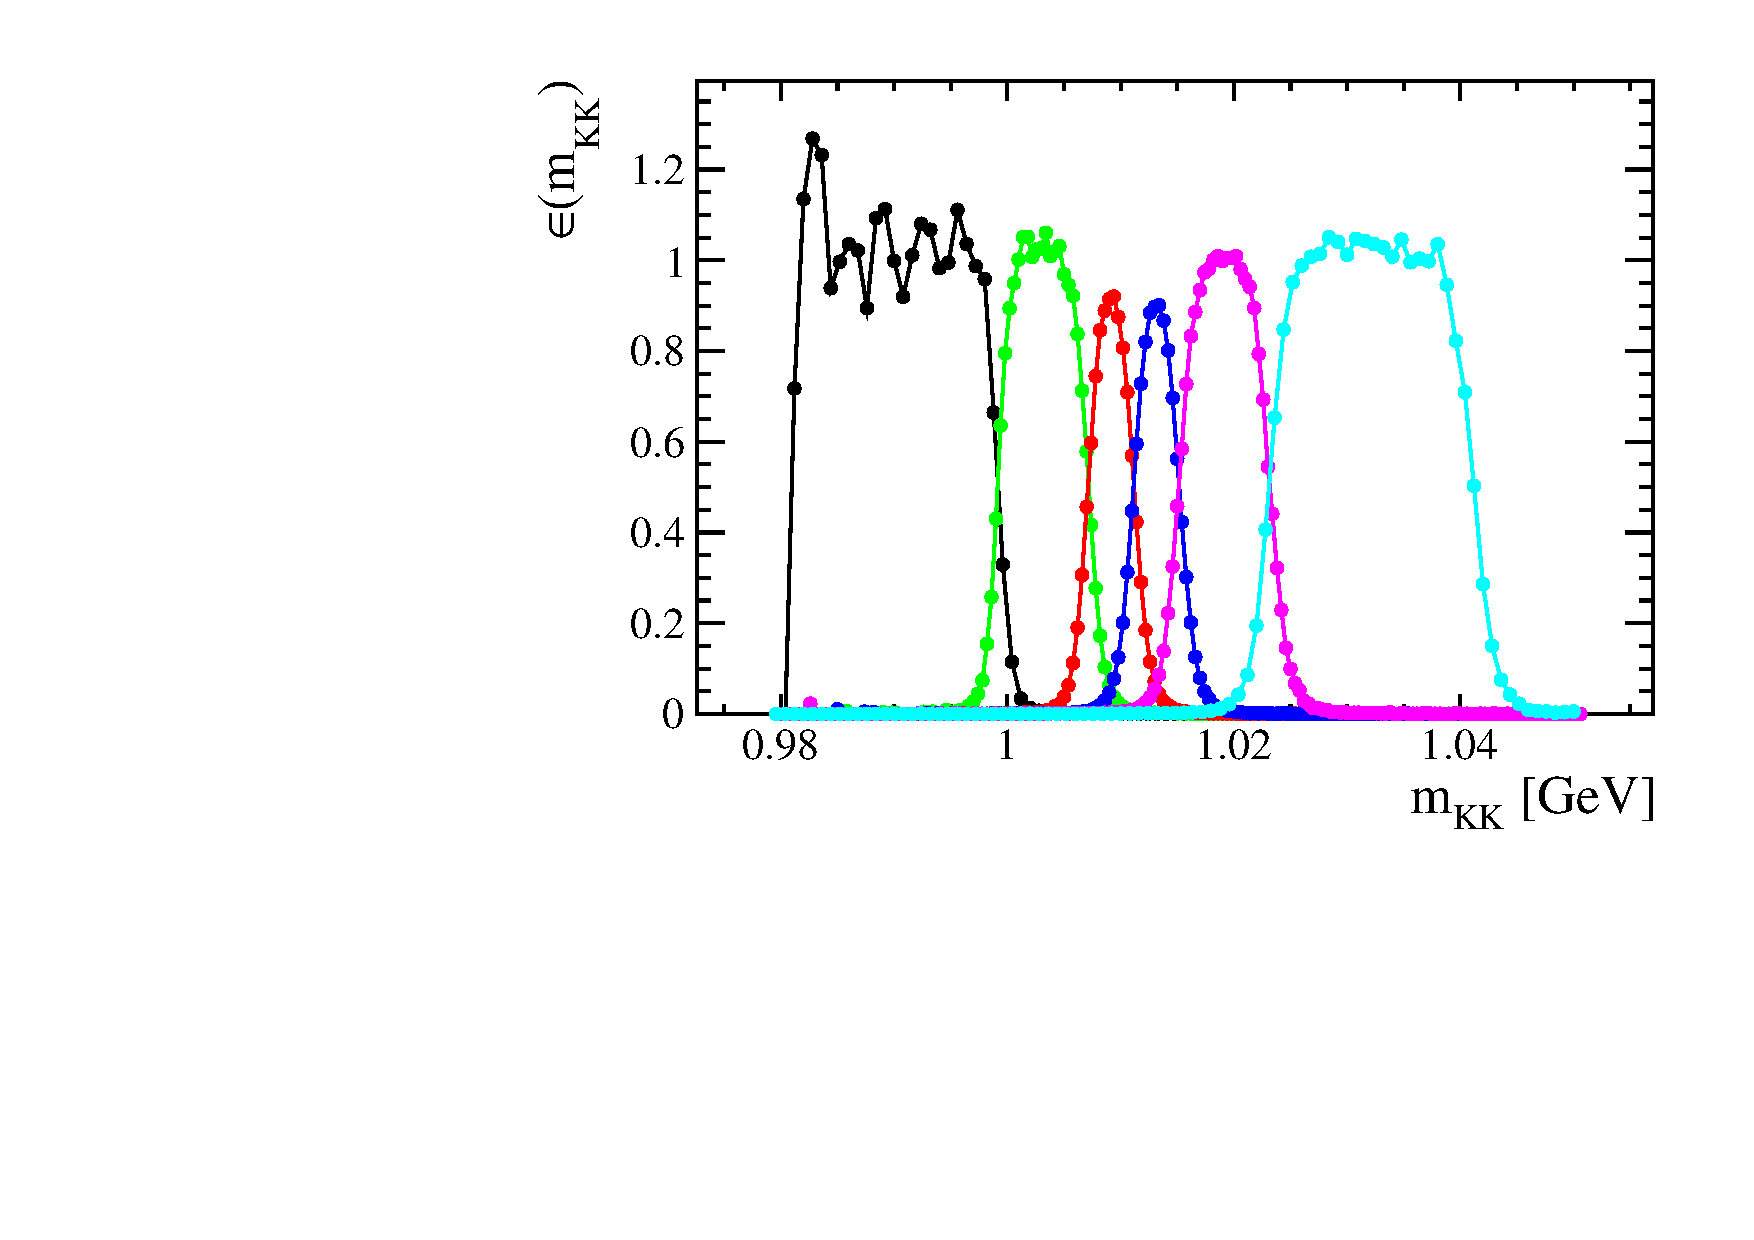
\includegraphics[width=0.49\textwidth]{figs/epsmKK.pdf}
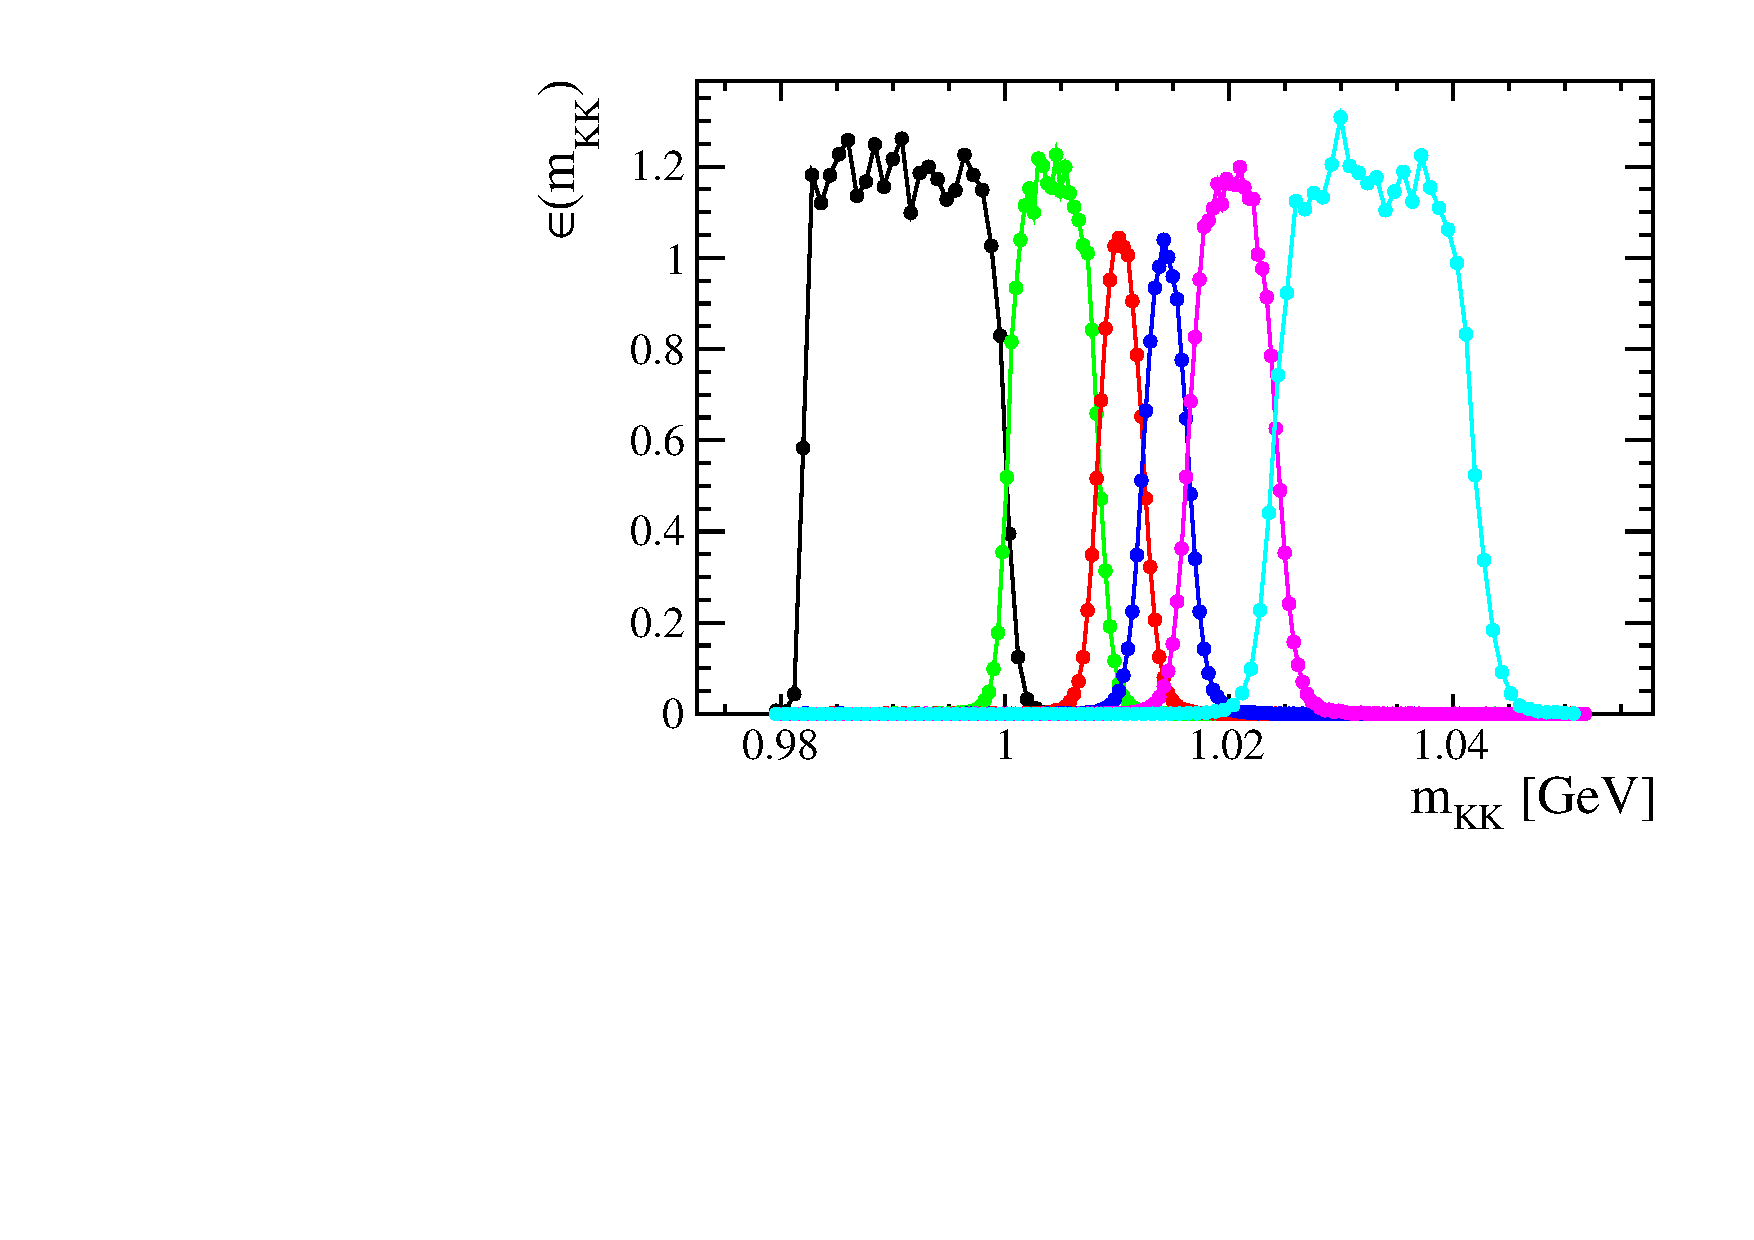
\includegraphics[width=0.49\textwidth]{figs/epsmKK_SWave.pdf}
\caption{\small Efficiency of each \mKK bin selection as a function of MC true \mKK using MC without (left) and with (right) S wave.}
\label{fig:epsilon_m}
\end{center}
\end{figure}

\begin{table}[h]
        \caption{$C_{\rm SP}$ factors obtained using Eq.~\eqref{eq:Csp2}. The $\phi$ resonance is parametrized with a relativistic Breit-Wigner.}
        \begin{center}
        \begin{tabular}{c|c}
                                              & \multicolumn{1}{c}{S-wave line shape}\\
                                                \hline\\
%                 \mKK bin             & Spline S-wave&$f_0(980)$& Unsmeared $f_0(980)$ \\ \hline
                $m_{KK}$ bin             &$f_0$ \\ \hline
                1         	        & 0.8569 \\
                2                    & 0.8768  \\
                3                    & 0.8478  \\
                4                    & 0.8821  \\
                5                    & 0.9406  \\
                6                    & 0.9711  \\
        \end{tabular}
        \label{tab:CSP1}
        \end{center}
\end{table}

\subsection{Decay time resolution}
An effective single-Gaussian model is used to parametrize the decay time resolution. This is sufficient to describe the damping effect of the time resolution. It is defined as follows, % It also allowed for a simple determination of systematic uncertainties since no multiple correlated parameters need to be varied
\begin{equation}
    \mathcal{P}(t) = \mathcal{R}(t) \otimes
    \left[ f_{\mathrm{prompt}}\delta(t) + 
    f_{\mathrm{ll}} \left(f_{\mathrm{sl}}e^{- t / \tau_s} + (1 - f_{\rm sl})e^{- t / \tau_{\rm l}}\right)
    \right] + f_{\mathrm{wpv}} W(t),
    \label{eq:decay_time_pdf}
\end{equation}
Where $t$ is the decay time, $\delta_t$ the decay time uncertainty (both calculated from  decay tree fit in which the PV position is constrained without constraining the $J/\psi$ mass). This model is fitted to $t$ in ten bins of $\delta_t$, with ${\cal R}(t)$ being:
        \begin{equation}
            {\cal R}(t) \propto \sum_{i=1}^{3} f_i \frac{1}{\sqrt{2\pi}\sigma_i} e ^{-\frac{1}{2}\left(\frac{t-\mu}{\sigma_i}\right)^2},
        \label{eq:decay_time_res_model}
        \end{equation}
where $\sum_i f_i =1$.
The three Gaussians have a common mean, different widths and two relative fractions, which are allowed to vary in the fit, as are the lifetime and relative fractions of the exponential functions. Another component corresponding to events with a wrongly-associated PV is added, the fraction of which is allowed to float in the fit. In each bin of $\delta_t$, the dilution of the triple Gaussian model is computed as,
\begin{equation}
    \label{eqn:time_dilution_tr}
    D = \sum_{i=1}^{3}f_i e^{-\sigma_i^2\Delta m_s^2/2},
\end{equation}
and the effective single Gaussian width as,
\begin{equation}
    \label{eqn:time_eff_res_tr}
    \sigma_{\rm eff} = \sqrt{(-2/\Delta m_s^2)\ln D},
\end{equation}
where $\Delta m_s = 17.77 \rm ps^{-1}$. This converts the resolution into a single-Gaussian function with an effective resolution that causes the same damping effect on the magnitude of the $B_s^0$ oscillation. A linear or quadratic calibration curve is then fitted to the variation of the effective resolution as a function of $\langle\delta_t\rangle$ to determine the calibration parameters. 
%% Parameterization of the resolution model
For calibration, simulated $B_s^0 \rightarrow J/\psi \phi$, prompt $J/\psi$ and inclusive $J/\psi$ samples are used, as well as prompt $J/\psi$ data.
The main source of systematic uncertainty in the calibration of the decay time resolution model is the translation from the prompt background sample to the signal sample. In addition, there is a systematic arising from the choice to include or not the
wrong-PV component.

%%A simulated $B_s^0 \rightarrow J/\psi \phi$ sample is used as calibration. A quadratic dependence on $\delta_t$ is assumed for $\sigma_{\rm eff}$,
%\begin{equation}
%    \label{eqn:time_res_tr}
%    \sigma_{\rm eff}(\delta_t) = p_0 + p_1\langle\delta_t\rangle + p_2\langle\delta_t^2\rangle,
%\end{equation}
%being the fitted values of the calibration constants  $p_0 = 0.00810 \pm 0.00018 \rm ps$, $p_1 = 0.731 \pm 0.011$ and $p_2 = 3.29 \pm 0.15 \rm ps^{-1}$. This calibration corresponds to an effective (single-Gaussian) resolution of $40.96 \pm 0.03 \pm 0.04 \rm fs$ in the
%selected and background-subtracted $B_s^0 \rightarrow J/\psi \phi$ data sample, where the first uncertainty is statistical from the %size of the $B_s^0 \rightarrow J/\psi \phi$ data sample and the second from the uncertainties on the calibration parameters. % MC2015 + MC2016
%A calibration using the simulated inclusive $J/\psi$ sample yields a 0.1\% difference in $\sigma_{\rm eff}$ with respect to the former case. Such difference is asssigned as a systematic uncertainty on the decay time resolution coming from translating the resolution from the prompt sample to the signal sample.

\subsection{Angular acceptance}
\label{subsec:AngAcc}
The angular acceptance is modelled using \textit{normalization weights} (see Ref.~\cite{LHCb-ANA-2012-067}, Sec.~3.3) obtained from fully simulated signal events from the Sim09b production. This simulation sample is iteratively weighted to match the distributions of final-state particle kinematics in the real data, as well as to match the physics parameters obtained from data, in order to correct for imperfections in the detector simulation. In order to do this, a GB reweighting is first applied in $p(B_s^0)$, $p_T(B_s^0)$ and $m(K^+K^-)$, together with a reweighting in $p(K^{\pm})$, $p_T(K^{\pm})$. The angular normalizations are computed, and the process is repeated until convergence is achieved (after 4 iterations).  

A total of 10 normalization weights are computed for each year and trigger category, as indicated in table \ref{tab:angAccWeightsComb}, where the combined weights are shown. The factorization of angular acceptance and decay time acceptance is assumed. A systematic effect is assigned to such assumption, comparing the final acceptance normalization weights obtained in six equal populated decay time bins.

\begin{table}[hbtp]
 \caption{\small Angular acceptance weights determined from all available Monte Carlo samples. The $f_k$ are the normalizations of the angular functions (see Equation~\ref{eq:rate_mult_lambda}) including the acceptance. They are used in the normalization of the \textit{p.d.f.}} \label{tab:angAccWeightsComb}
 \center
\resizebox{\linewidth}{!}{
%\input{tex/AngAccTables/AngularAcceptanceTable_trigYearComp_2015_2016_IncldDG0_BKGCAT_0_50_60_sigmat015_XM_BP_BPT_KmpPTP_FirstKin_SepWeighting_16042018_fi__IncldG0_initial.tex}
\begin{tabular}{r l |c c c c}
\hline
& $k$ & \multicolumn{4}{c}{$f_k/f_1$}\\\hline
&     & \multicolumn{2}{c}{$2015$} & \multicolumn{2}{c}{$2016$} \\\hline
&     & ``Unbiased trigger"  & ``Biased" trigger & ``Unbiased trigger"  & ``Biased trigger"\\
\hline
1 & (00)                   &  $1  \pm 0$           &  $1\pm0$ & $1  \pm 0$           &  $1\pm0$ \\
2 & ($\parallel\parallel$) & $1.0297\pm0.0019$ & $1.0278\pm0.0036$ & $1.02637\pm0.00079$ & $1.0181\pm0.0017$\\
3 & ($\perp\perp$) & $1.0299\pm0.0019$ & $1.0280\pm0.0035$ & $1.02590\pm0.00078$ & $1.0184\pm0.0017$\\
4 & ($\parallel\perp$) & $-0.0007\pm0.0015$ & $-0.0071\pm0.0030$ & $-0.00029\pm0.00063$ & $0.0017\pm0.0015$\\
5 & ($0\parallel$) & $-0.00013\pm0.00090$ & $0.0038\pm0.0017$ & $0.00115\pm0.00038$ & $0.00260\pm0.00080$\\
6 & ($0\perp$) & $0.00119\pm0.00089$ & $0.0026\pm0.0017$ & $-0.00010\pm0.00038$ & $-0.00091\pm0.00079$\\
7 & (SS) & $1.0076\pm0.0013$ & $1.0123\pm0.0025$ & $1.00618\pm0.00054$ & $1.0112\pm0.0012$\\
8 & (S$\parallel$) & $-0.0005\pm0.0012$ & $-0.0008\pm0.0023$ & $0.00045\pm0.00048$ & $-0.0003\pm0.0010$\\
9 & (S$\perp$) & $-0.0008\pm0.0012$ & $0.0000\pm0.0023$ & $-0.00020\pm0.00049$ & $-0.0005\pm0.0010$\\
10 & (S0) & $0.0013\pm0.0024$ & $-0.0047\pm0.0047$ & $-0.0008\pm0.0010$ & $-0.0059\pm0.0022$\\
\hline
\end{tabular}
}
\end{table}
A cross-check has been performed using a sample of $B^+ \rightarrow J/\psi K^+$ decays in 2016 data, yielding a good consistency in the method. %% In this decay the muon helicity angle, $\theta$, exhibits a purely $\sin^2\theta$ dependence, which provides the benchmark against which the validity of the simulation can be tested. In particular, this study will investigate the behavior of the simulation correction as a function of $\eta(\Bu)$ since there are some issues with the performance of the simulation for charged tracks at low $\eta$.

\subsection{Decay time acceptance} 
\label{subsec:TimeAcc}
The reconstruction efficiency is not constant as a function of the $B^0_s$ decay time due to displacement requirements made on signal tracks in the trigger and event selection and to a decay-time-dependent efficiency to reconstruct the tracks in the VELO \cite{LHCb-PAPER-2013-065}. The overall decay-time acceptance is determined using the control channel $B^0 \to J/\psi K^{*}(892)^0$,
with $K^{*}(892)^0 \to K^+\pi^-$, which is kinematically very similar to the signal decay and it is assumed to have a purely exponential decay-time distribution with a well-known lifetime (i.e.the width difference $\Delta \Gamma_d$ is ignored), namely $1.518\pm 0.004$ ps\cite{HFLAV2017}.
The strategy to select $B^0 \to J/\psi K^{*}(892)^0$ events and compute the sWeights is similar to the one used for $B_s^0 \rightarrow J/\psi K^+ K^-$ events
The $K^+\pi^-$ system in the $B^0 \rightarrow J/psi K^+\pi^-$ decay can be in a relative S-wave or P-wave configuration. A $\sim6\%$ presence of S-wave has been observed in data, as described in~\cite{LHCb-PAPER-2013-023}. However, the simulated $B^0 \rightarrow J/\psi K^{*}(892)^0$ sample only includes the P-wave component. To account for this, an iterative procedure similar to the one described in \red{\ref{subsec:AngAcc}} is applied, reweigthing the simulation to match the $B^0$ $p$ and $p_T$, as well as $m(K^+\pi^-)$ distributions in data. %%\red{revisar}

The decay time acceptance is defined as
\begin{equation}
	\varepsilon_{\rm data}^{B_s^0}(t) = \varepsilon_{\rm data}^{B^0}(t) \times \frac{\varepsilon_{\rm sim}^{B_s^0}(t)}{\varepsilon_{\rm sim}^{B^0}(t)},
\label{eq:timeacc}
\end{equation}
where $\varepsilon_{\rm data}^{B^0}(t)$ is the efficiency in data of the fully triggered, selected and sweighted events in the $B^0$ control channel and $r(t)=\varepsilon_{\rm sim}^{B_s^0}(t)/\varepsilon_{\rm sim}^{B^0}(t)$ is the ratio of efficiencies of the
simulated signal and control modes after the full trigger, selection and MC-data correction chain has been applied.
This second term in the acceptance, $r(t)$, accounts for the small differences in the lifetime and kinematics between
the signal and control modes. The MC events are reweighted to match the $p.d.f.$ of the respective data. %%\red{more?} 

To derive $\varepsilon_{\rm data}^{B_s^0}(t)$ a simultaneous fit is performed to both the simultaneous samples and the data control channel. This allows to have the overall uncertainties on the $B^0_s$ data spline coefficients, thus providing an easier control on the associated systematic uncertainty. The decay time acceptance $\varepsilon_{\rm data}^{B_s^0}(t)$ is then used in the fit to the $B^0_s$ data signal sample to determine the physics parameters.

For the $B^0$ and $B_s^0$ the model used for the fit is composed of the product of a single exponential, convoluted with a single Gaussian resolution, and the respective acceptance function. The latter is modelled using cubic splines with knots at [0.3, 0.58, 0.91, 1.35, 1.96, 3.01,12.00] $\ps$ and the first coefficient is fixed to unity. The knot positions have been chosen according to an exponential distribution between [0.3,15] ps in order to have six equally populated bins considering $\Gamma=0.66\ps$. The last knot position is moved from 15 $\ps$ to 12 $\ps$ in order to have stable fits also for the trigger-year categories which have no decay candidates at these large decay times.

In order to obtain a single spline, $s_{data}^{B_s^0}$, that represents $\varepsilon_{\rm data}^{B_s^0}(t)$, combinations of the following three splines are used to describe the acceptance of the three datasets:
\begin{itemize}
\item One spline representing the acceptance in $B_s^0$ MC: $s_{sim}^{B_s^0}$
\item One spline representing the ratio of acceptances in $B^0$ and $B_s^0$ MC: $s_{sim}^{B^0/B_s^0}$
\item One spline representing the final acceptance in $B_s^0$ data: $s_{data}^{B_s^0}$
\end{itemize}
These splines are used in the following combinations to describe the acceptances for the three datasets:
\begin{itemize}
\item $B_s^0$ MC: $s_{sim}^{B_s^0}$
\item $B^0$ MC: $s_{sim}^{B^0/B_s^0} \times s_{sim}^{B_s^0}$
\item $B^0$ data: $s_{data}^{B_s^0} \times s_{sim}^{B^0/B_s^0}$
\end{itemize}

A single Gaussian models the resolution, and has a mean of 0$\rm ps$ and a width of 42$\rm fs$/39$\rm fs$/42$\rm fs$ for $B_s^0$ MC/$B^0$ MC/$B^0$ data, motivated by the studies in Section~\ref{sec:timereso} and the difference of the resolution between $B_s^0$ and $B^0$ seen in truth matched MC. The lifetime in the fit is fixed to the World average value for data $\tau_{B^0}^{\mathrm{data}} = 1.518\,\rm ps$~\cite{HFLAV2017}, and to the value used in the generation of the MC for the simulated samples, namely $\tau_{B^0}^{\mathrm{MC}} = 1.519\,\rm ps$ and $\tau_{\B^0_s}^{\mathrm{MC}} = 1.512\,\rm ps$.

The decay time acceptance is obtained separately for the data taking periods 2015 and 2016 and two different trigger paths (``unbiased" and ``exclusively biased"). 
\red{plots?}

The lifetimes $\tau(B^{0})$ and $\tau(B^{+})$ in $B^{0}\to \jpsi K^{*0}$ and $B^{+}\to \jpsi K^{+}$ decays are measured as a crosscheck of the time acceptance procedure. 2016 data and simulation samples for both validation channels are used.  The same procedure as for $B^{0}_{s}\rightarrow J/\psi \phi$ is used, including the spline knot positions and time resolution (see \secref{sec:timeAcc_timeaccBd}).

\subsubsection{Measurement of $\tau(B^{0})$} 

The procedure to determine the decay time efficiency (\secref{sec:timeAcc_timeaccBd}) is validated by splitting the 
$B^{0}\to\jpsi K^{*0}$ control sample (both data and simulation) into two independent sets. One half of the sample is then used as a control while the other is used to measure $\tau(B^0)$.
Three different criteria are considered for this, namely:
% Different splittings
\begin{itemize} 
    \item Splitting according to odd/even eventNumber in the
        original sample, where the sample that is used instead of $B_s^0$ has a
    cut on $\delta_t < 0.04\rm ps$.  
\item Splitting according to odd/even
        eventNumber in the original sample, where the sample that is used for
        fitting has a cut on the opening angle between the kaon and the pion
        that come from the $K^{*0}$, angle $<$ 0.025 rad. The position of the cut is
        chosen such that the average of the opening angle distribution is close
        to the corresponding one for the $B^{0}_{s}\to J/\psi \phi$ sample.
    \item Splitting on the $K^{*0}$ mass: events with $m(K^{*0}) < 890\ \rm
        GeV/{c^2}$ are used for fitting, events with $m(K^{*0}) > 890 \ \rm
        GeV/{c^2}$ are used as control sample.  
        \end{itemize}

For the control samples, the $B^{0}$ lifetime is fixed to its input for
simulation (1.519 ps) and to the
world average value for data (1.518 ps)~\cite{HFLAV2017}. We obtain the values
listed in the first column of \tabref{tab:tauB0}, where the deviation from the
world average ~\cite{HFLAV2017} is also shown. To
further improve these results, we also try reweighting the simulated samples according
such that the \Bd meson \pt distribution matches that in data,
as shown in \figref{fig:B0_PT_rew}.
The corresponding values for the lifetime (second column of \tabref{tab:tauB0})
show a better agreement with the PDG value. The fits to the decay time
distribution with MC reweighting in \pt for the different splittings are
shown in~\figref{fig:B0_tau_fit}.

Finally, a reweighting that takes into consideration the S-wave fraction present in
data (in addition to the aforementioned MC reweighting in $B^0$ \pt) is also
considered. %, using the results from Section~\ref{sec:Bd_swave}.
The splitting that is applied is the one depending on the $K^{*0}$
mass. The corresponding fitted lifetime is found to be  $\tau(\Bd) =
1.519\pm0.006$\ps, 0.13$\sigma$ (0.05\%) from the world average~\cite{HFLAV2017},
thus showing a good agreement. The fitted decay time is shown in
\figref{fig:B0_tau_fit}. 

\begin{table}[th]
\caption{\label{tab:tauB0}\small Values of $\tau(B^{0})$ obtained for validation of the time acceptance method for the different considered splittings, with (first column) and without reweighting MC in $p_{T}^{B}$.}
\centering{
\begin{tabular}{c|c|c}
    Splitting   & No $B^0$ $p_T$ reweighting & $B^0$ $p_T$ reweighting    \\
    \hline
   	$\delta_t < 0.04\rm ps$       & $1.482 \pm 0.007\rm ps$ (5.21$\sigma$,2.35\%)  & $1.518 \pm 0.007\rm ps$ (0.05$\sigma$,0.03\%)               \\ 
    angle $< 0.025\rm rad$     & $1.522 \pm 0.008\rm ps$ (0.52$\sigma$,0.28\%) & $1.523 \pm 0.008\rm ps$ (0.57$\sigma$,0.31\%)                  \\
    $m(K^{*0})$  & $1.518 \pm 0.006\rm ps$ (0.02$\sigma$,0.01\%) & $1.518 \pm 0.006\rm ps$ (0.03$\sigma$,0.01\%) 
\end{tabular}
}
\end{table}

% Plots with the reweighting 
\begin{figure}[tb!]
\centering{
    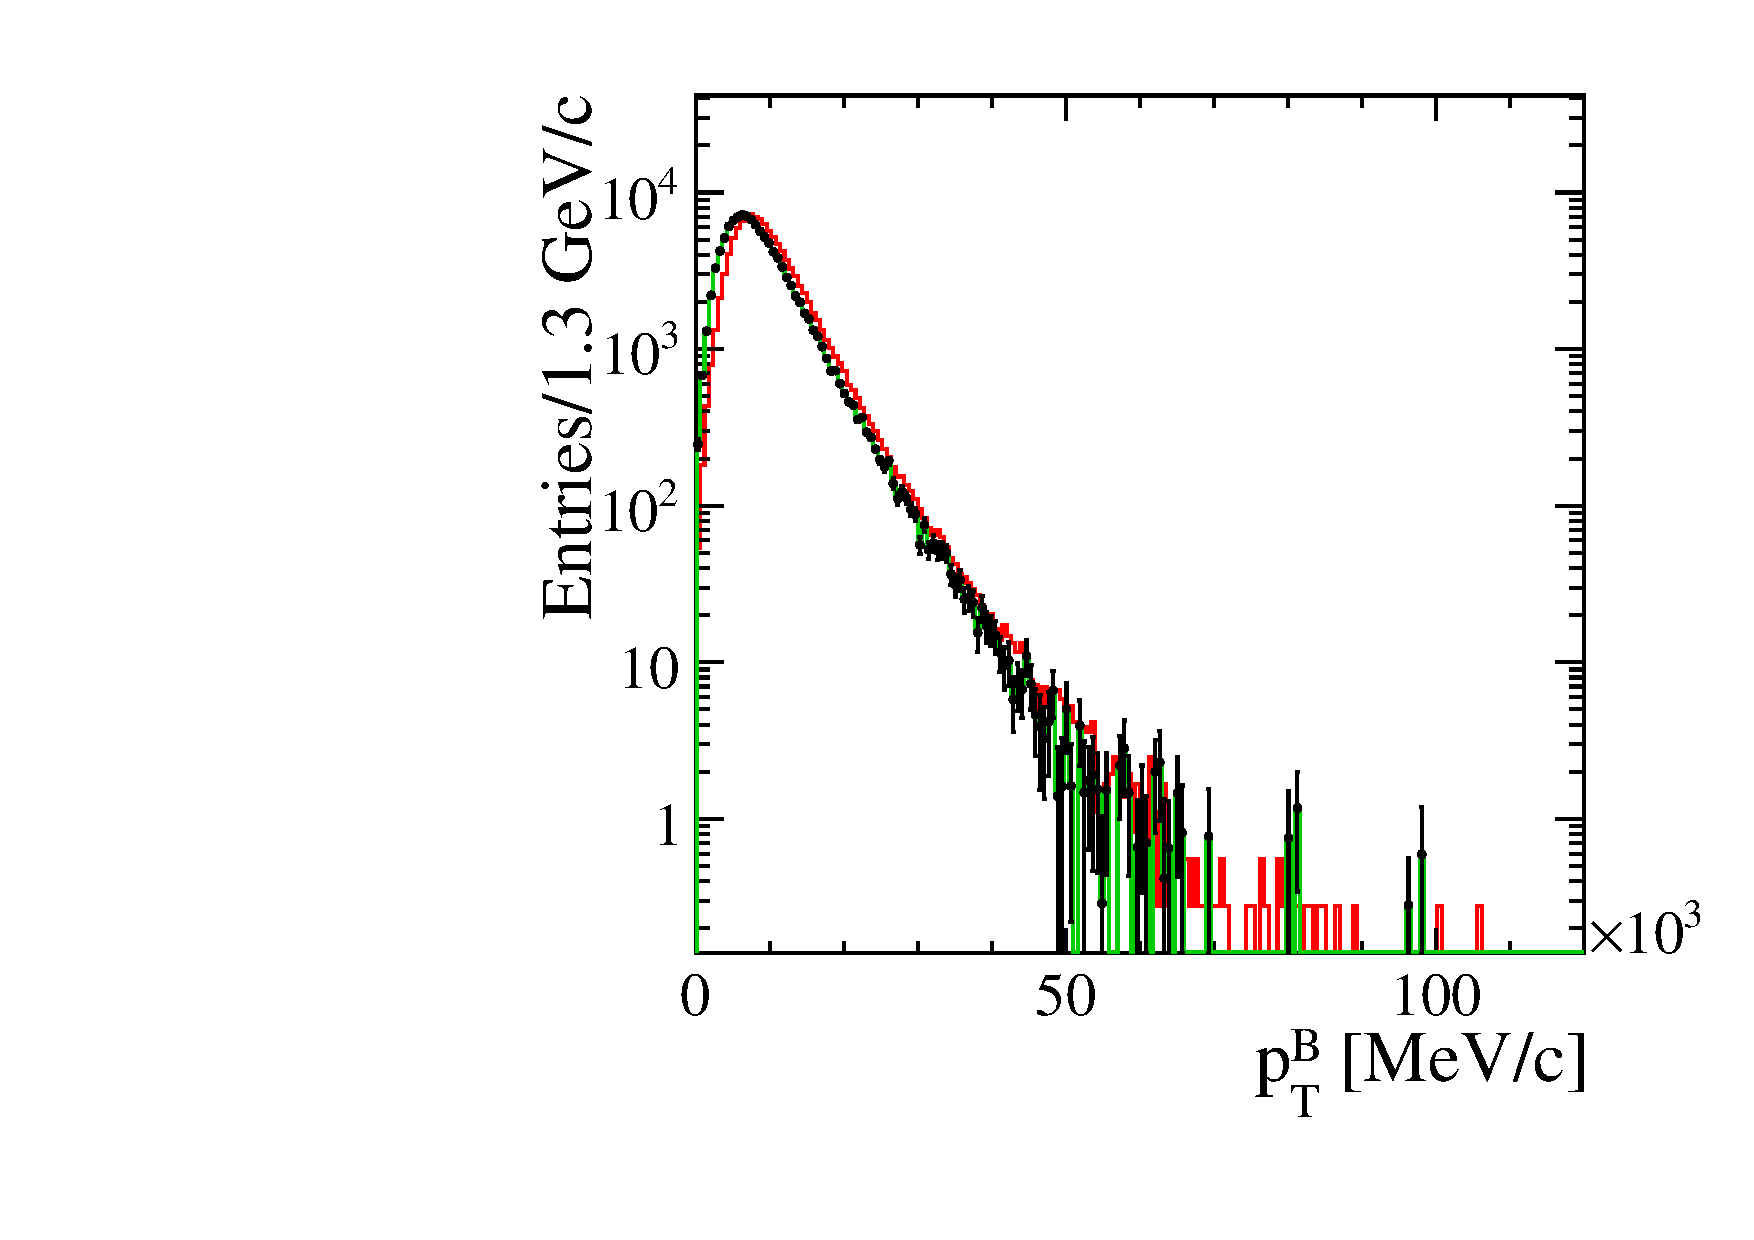
\includegraphics[width=0.29\textwidth]{figs/timeacc/B0_PT_reweighted_SigmaCut.pdf}
    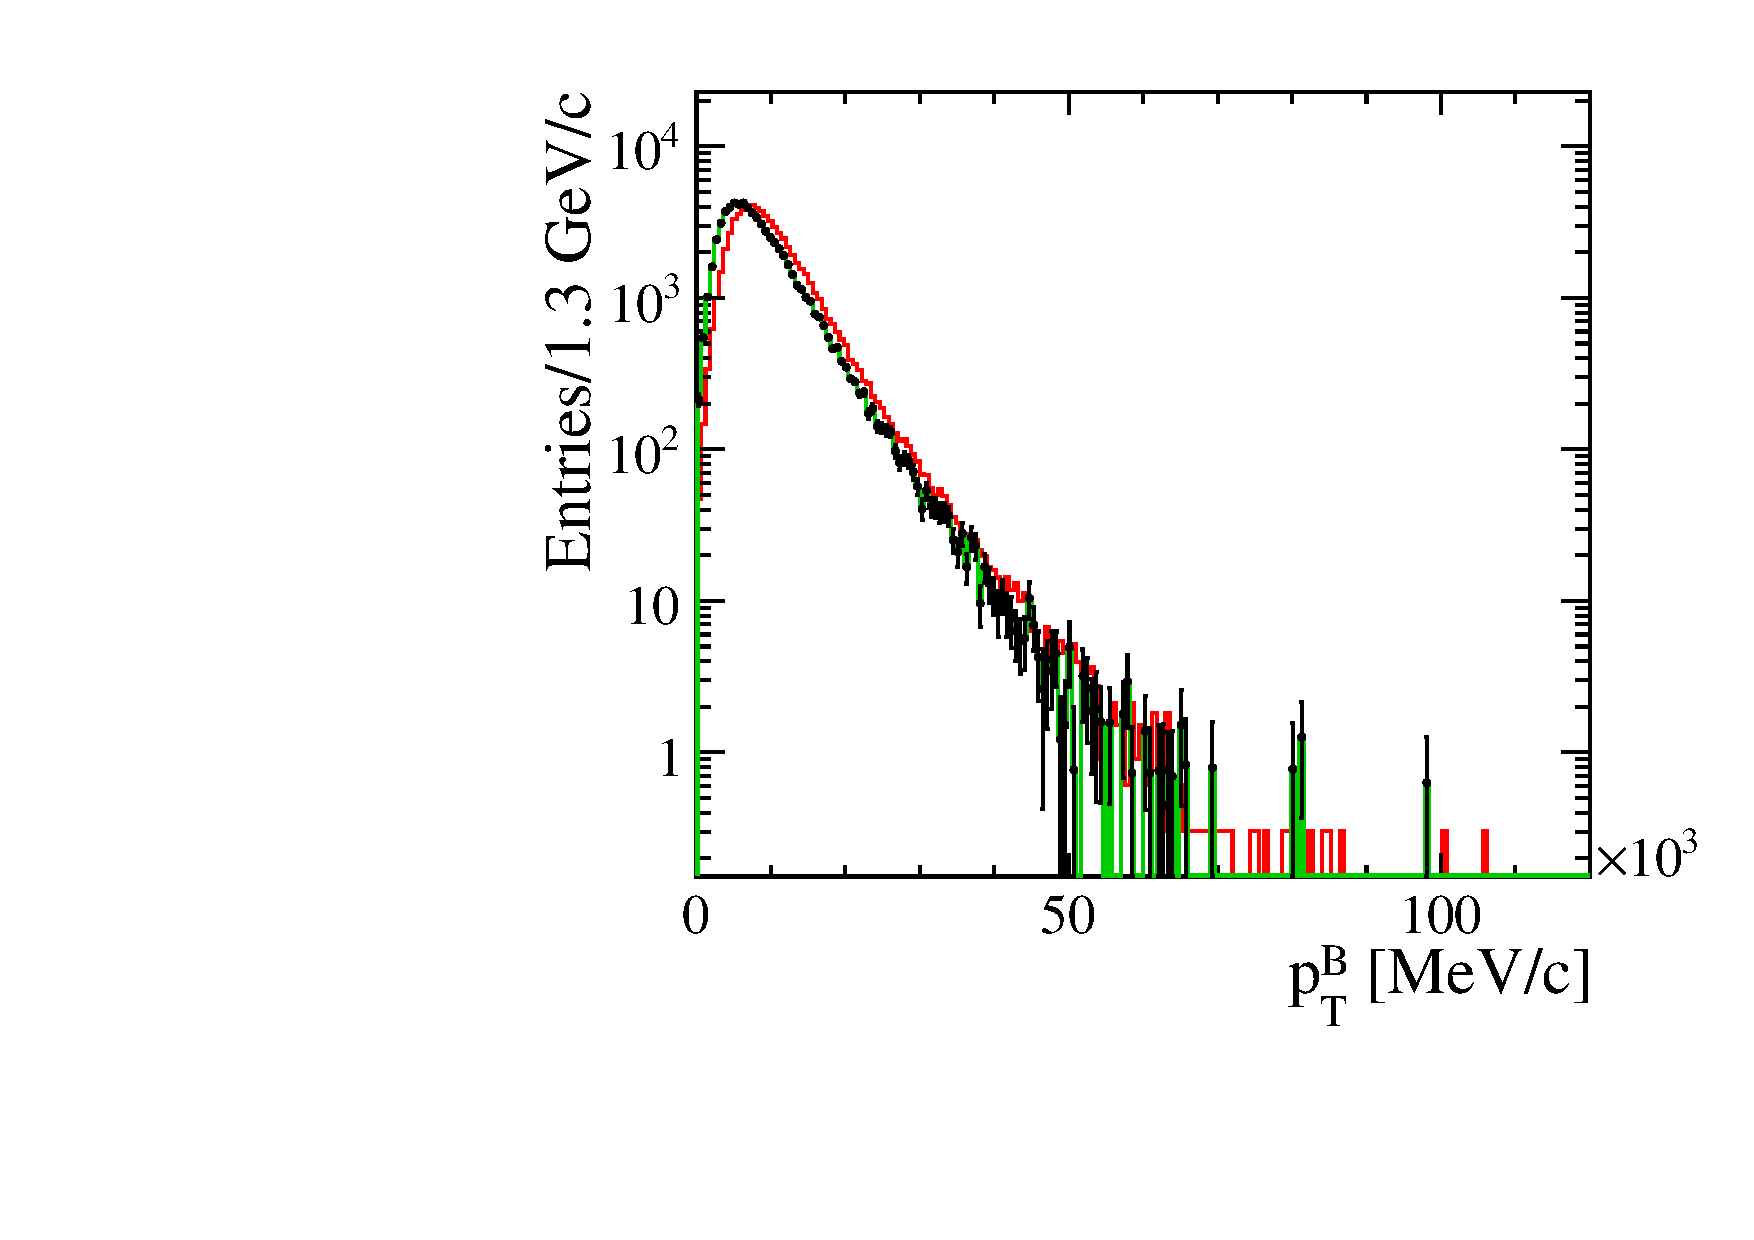
\includegraphics[width=0.32\textwidth]{figs/timeacc/B0_PT_reweighted_AngleCut.pdf}
    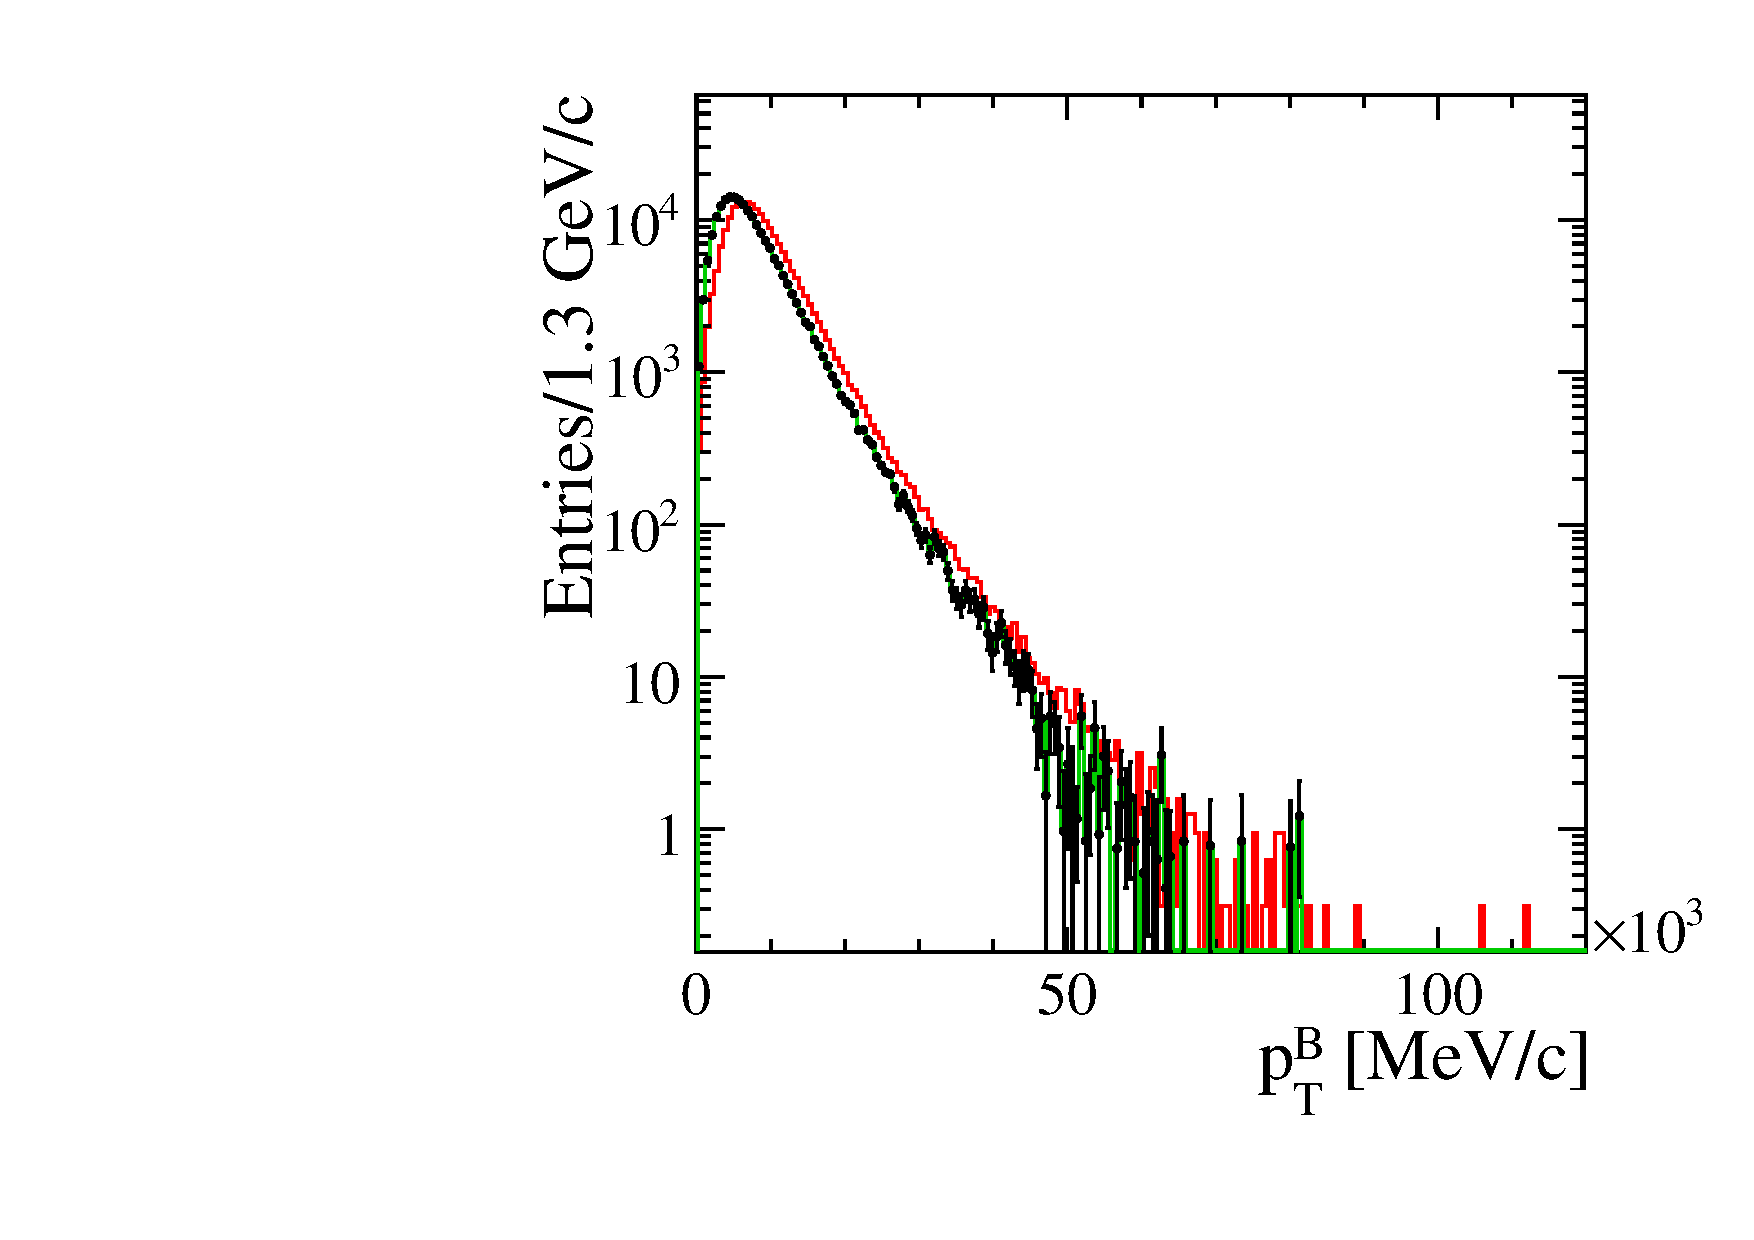
\includegraphics[width=0.31\textwidth]{figs/timeacc/B0_PT_reweighted_MassCut.pdf}
	\caption{\small Distributions of $p_{T}^{B}$ for $B^{0}\to J/\psi K^{*0}$ using splitting according to eventNumber with $\sigma_t < 0.04$ (top left) and angle $<$ 0.025 (top right), and splitting according to $m(K^{*0})$ (bottom). The black dots represent data and the red and green lines the MC before and after the reweighting, respectively.
    \label{fig:B0_PT_rew}
        }}
\end{figure}

% Plots of the fit 
\begin{figure}[tb!]
\centering{
    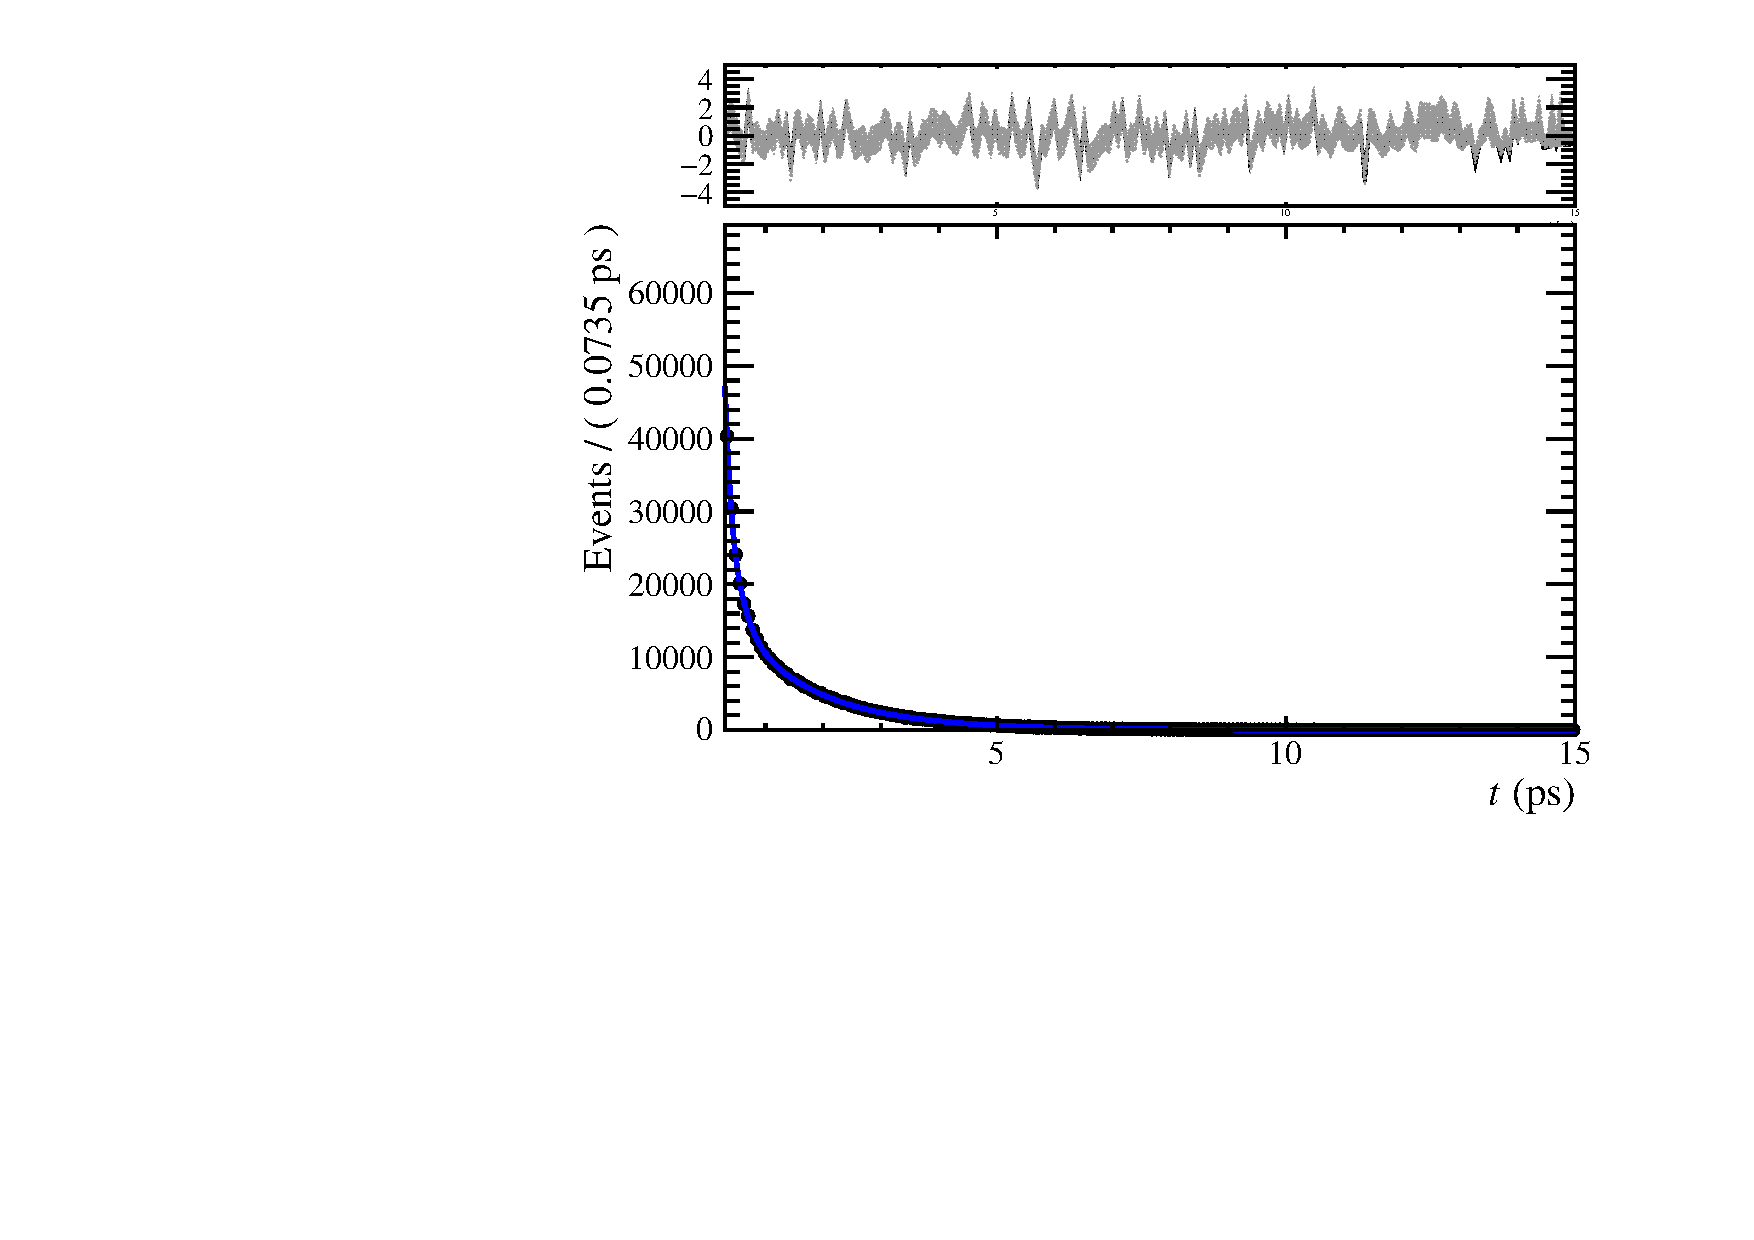
\includegraphics[width=0.4\textwidth]{figs/timeacc/B0_time_fits_reweighted_SigmaCut.pdf}
    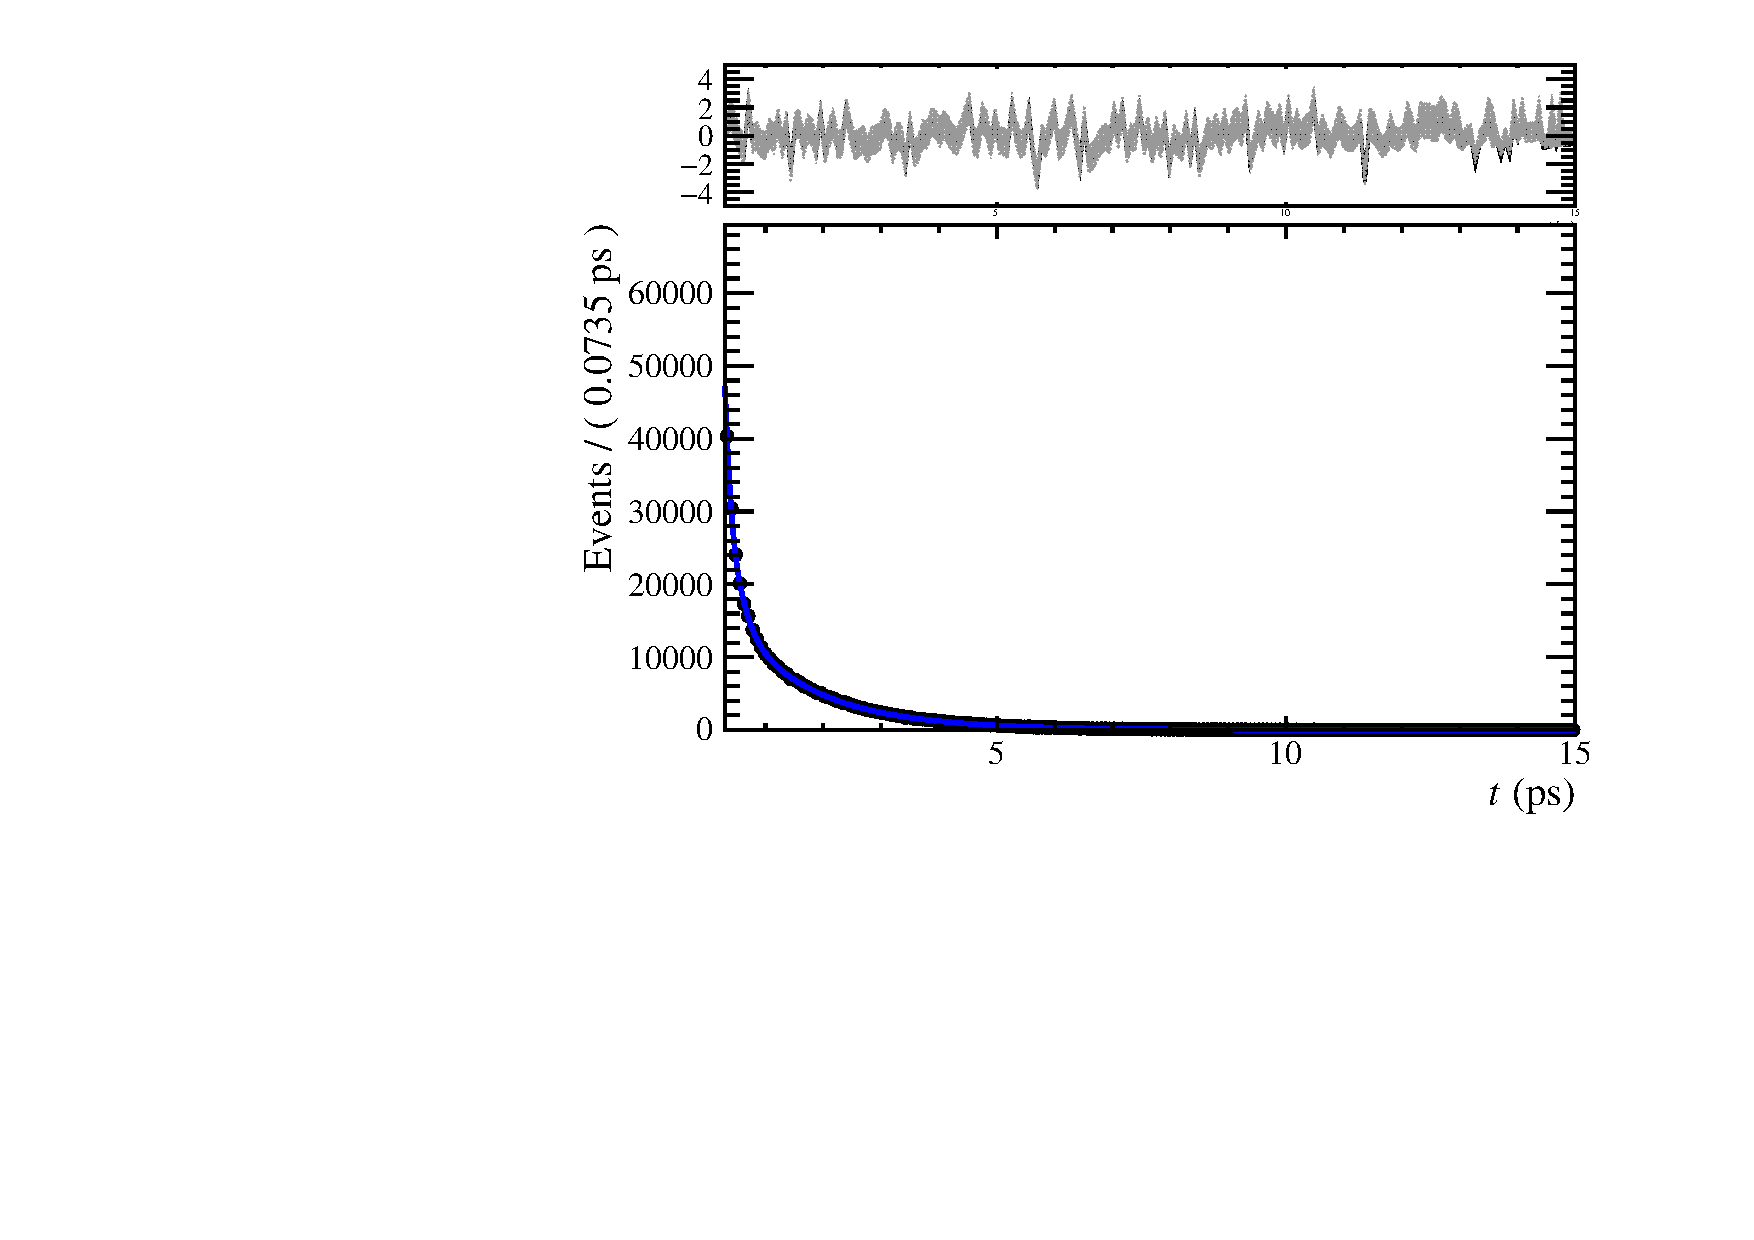
\includegraphics[width=0.4\textwidth]{figs/timeacc/B0_time_fits_reweighted_AngleCut.pdf}\\
    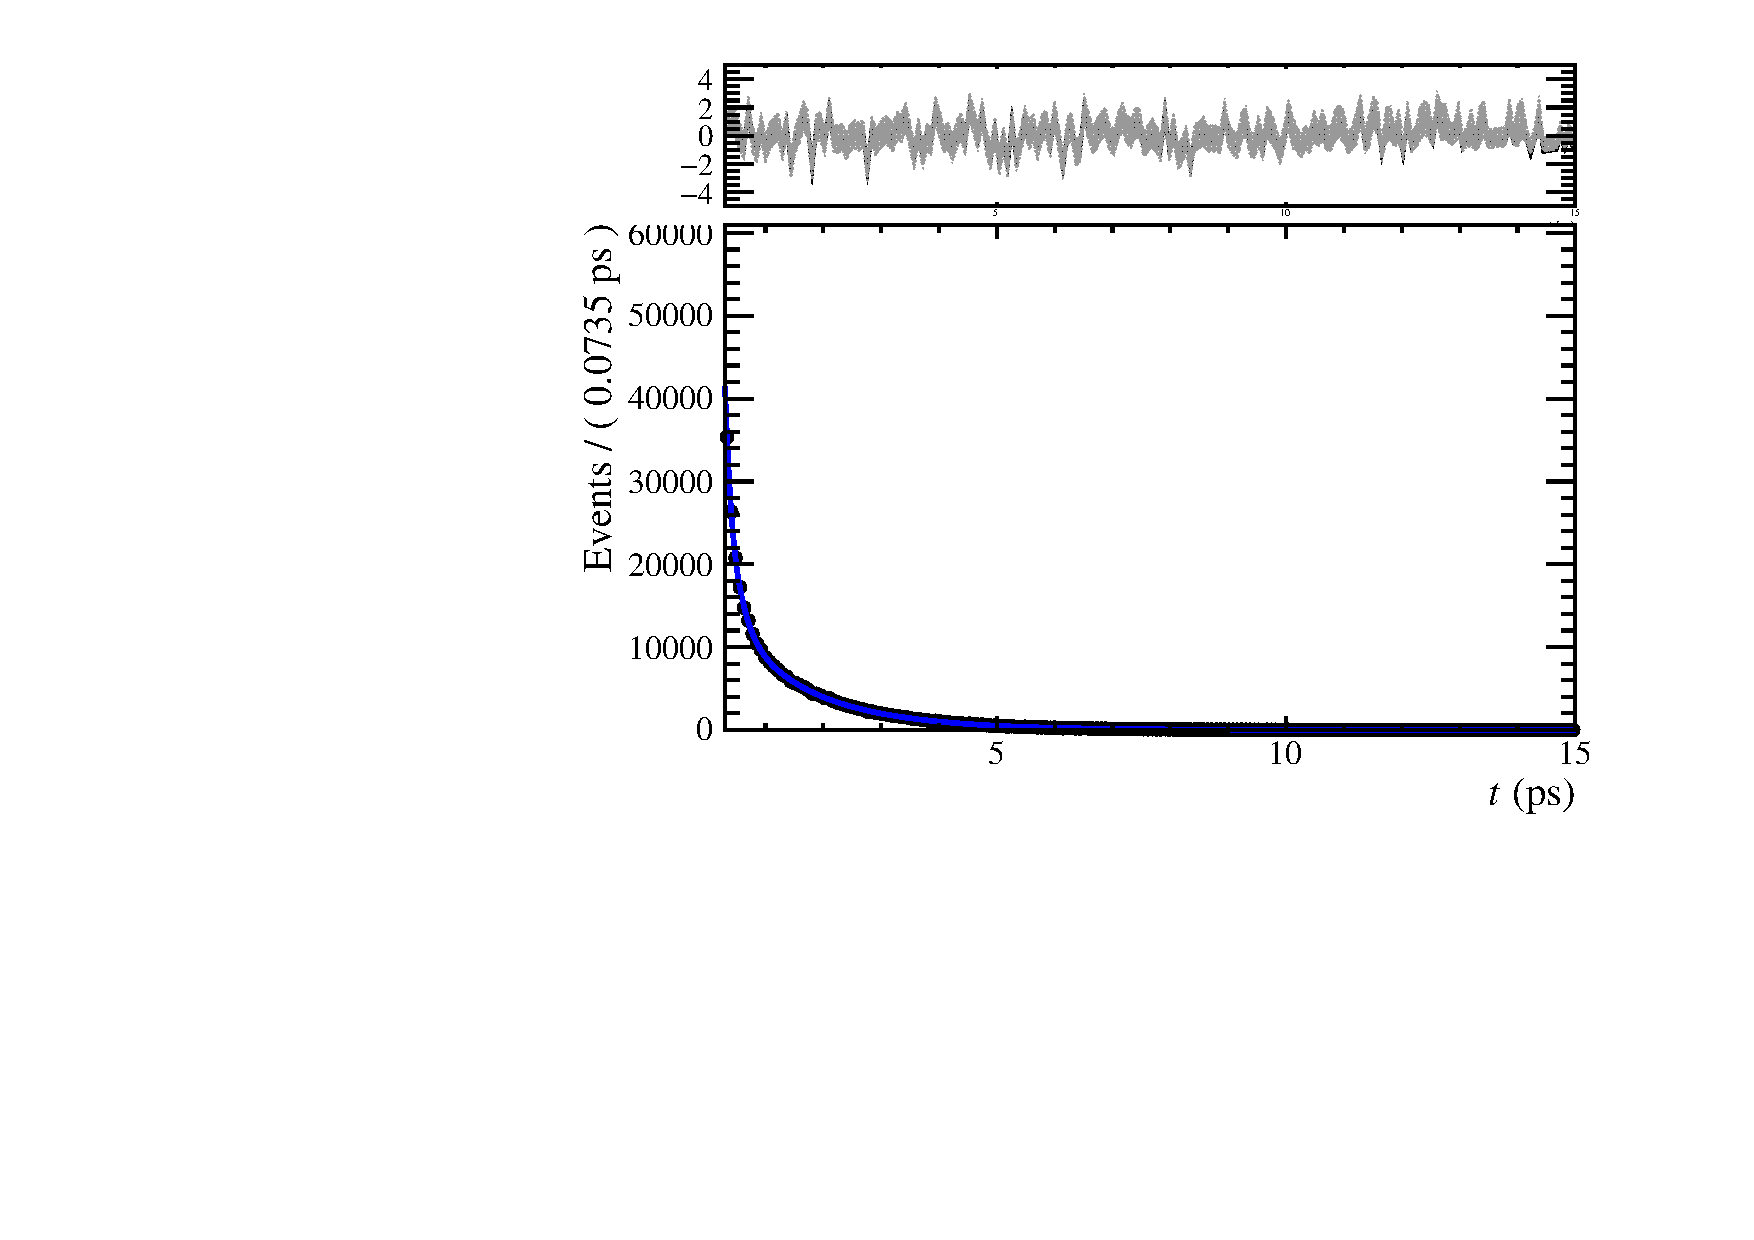
\includegraphics[width=0.4\textwidth]{figs/timeacc/B0_time_fits_reweighted_MassCut.pdf}
    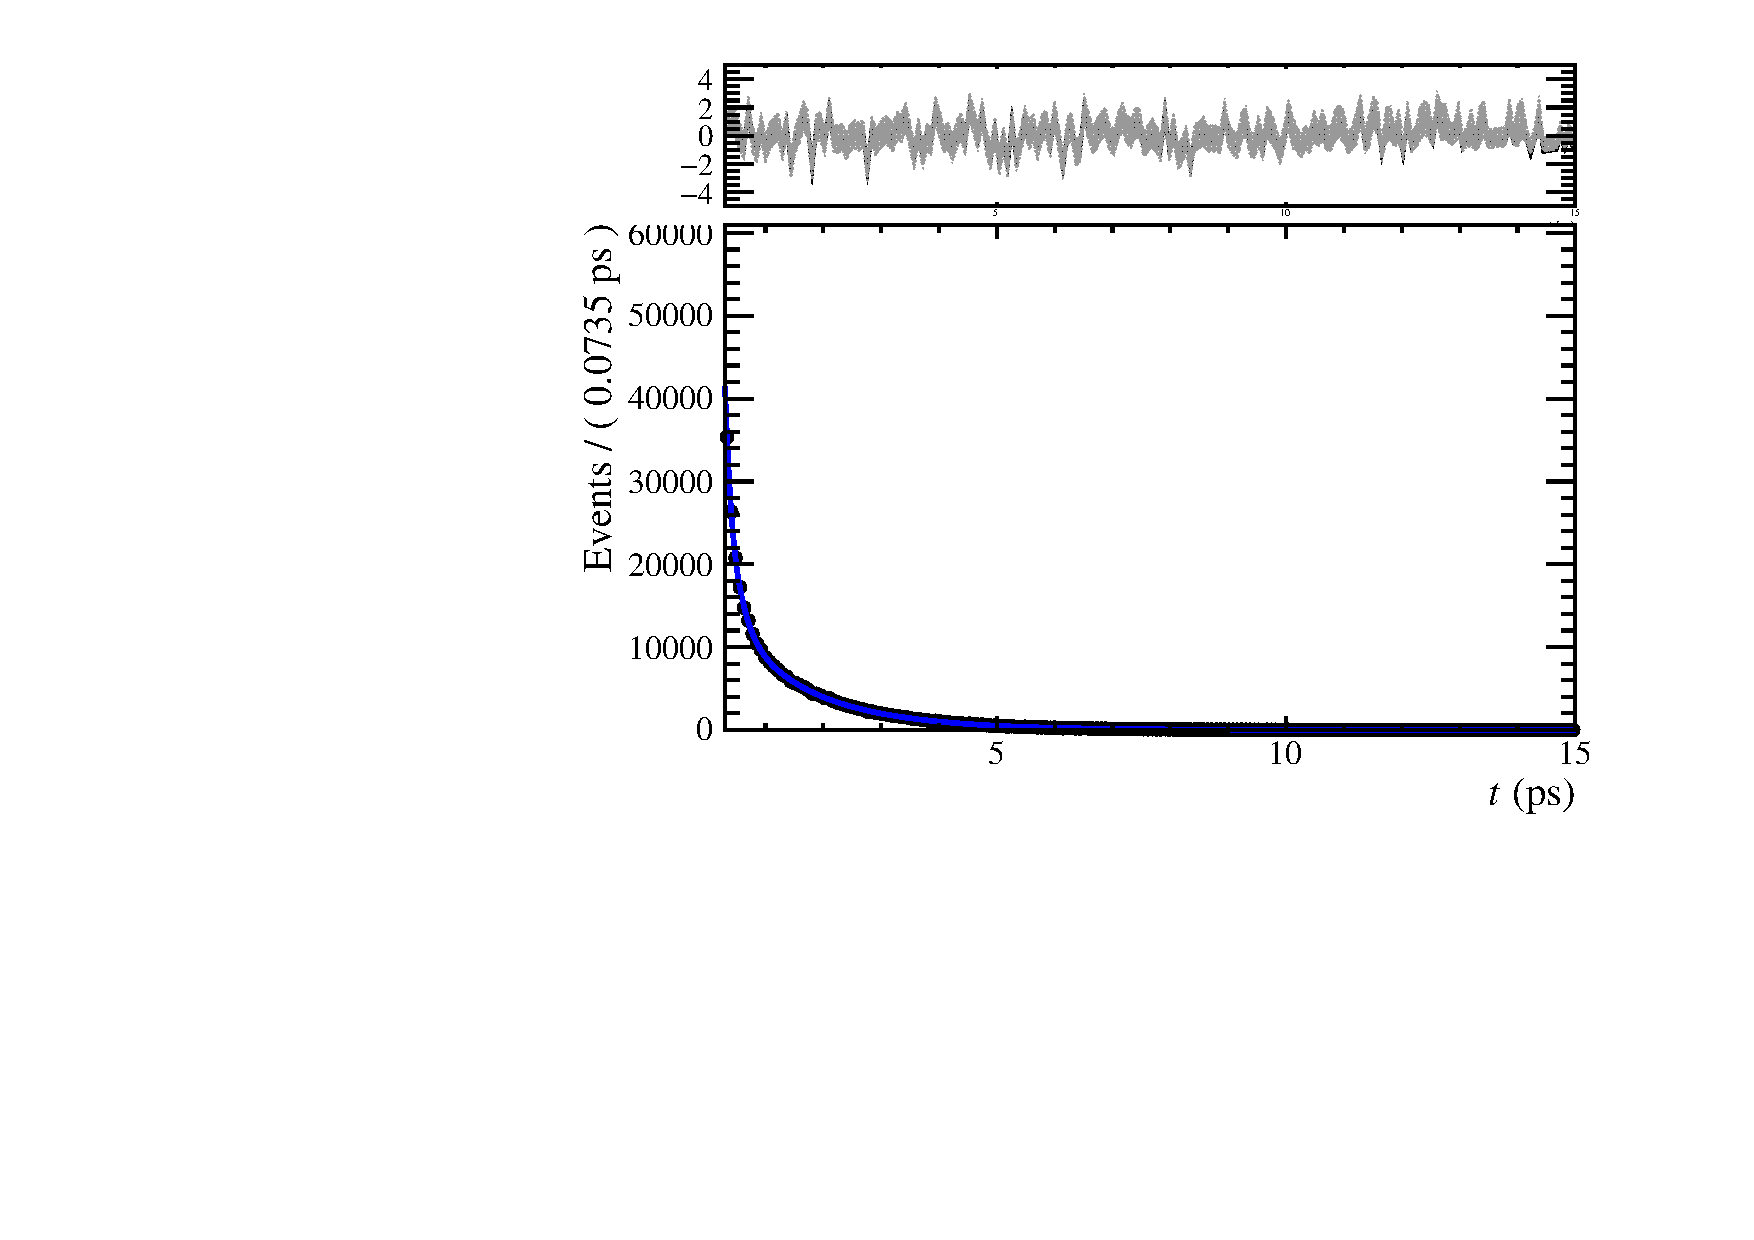
\includegraphics[width=0.4\textwidth]{figs/timeacc/B0_time_fits_reweighted_MassCut.pdf}
	\caption{\small Decay time distribution of $B^{0}\to J/\psi K^{*0}$ decays and the corresponding
    likelihood fit result,
    splitting according to eventNumber with $\sigma_t < 0.04$ (top left) and angle $<$ 0.025 (top right), and splitting according to $m(K^{*0})$ without (bottom left) and with S-wave consideration.
    \label{fig:B0_tau_fit}
        }}
\end{figure}

%%\red{uncertainties}

\subsection{Flavour tagging}
\label{subsec:Tagging}
%%% Tagging parameters constrained in final fit → systematics propagated into final result
For time-dependent studies the ability of properly identifying the initial flavour of the meson (known as \textit{flavour tagging}) is fundamental. To this end, two flavour tagging algorithms are used: the opposite-side (OS) taggers and the same-side kaon (SSK) taggers, which exploit specific features of the incoherent production of $b\bar{b}$ quark pairs in $pp$ collisions.

Each tagging algorithm gives a tag decision and a mistag probability, the fraction of events with the wrong tag decision, $\eta \in [0, 0.5]$. The tag decision takes values +1, 1, or 0, if the signal meson is tagged as $B_s^0$, $\bar{B}_s^0$ or untagged, respectively. The fraction of events in the sample with a nonzero tagging decision gives
the efficiency of the tagger, $\varepsilon$. The mistag probability is then calibrated to obtain the corrected per-event mistag probability, $\omega$. This is used to determine the dilution factor, $\mathcal{D} = (1 − 2\omega)$, that rescales the efficiency of the tagger to quantify the fraction of the sample equivalent to perfectly tagged events. This effective efficiency is called tagging power, given by the product of the efficiency and the square dilution, $\varepsilon\mathcal{D}^2$.

In this analysis the taggers have been optimised for Run 1 data but here their
calibration is determined using Run 2 data. \red{update if necessary} A linear dependence of $\omega$ with $\eta$ is assumed, 
\begin{equation}
\omega = p_0 + p_1(\eta - \left \langle \eta \right \rangle)
\end{equation}
where $p_0$, $p_1$ are calibration parameters and $\left \langle \eta \right \rangle$ is the average predicted mistag probabilities for the calibration samples. When using OS and SSK algorithms, the calibration model become:
\\
\begin{center}
$\omega^{\rm alg} = (p_0^{\rm alg} + \frac{\Delta p_0^{\rm alg}}{2}) + (p_1^{\rm alg} + \frac{\Delta p_1^{\rm alg}}{2})(\eta^{\rm alg} - \left \langle \eta^{\rm alg} \right \rangle)$ for an initial $B_s^0$ event 
\end{center}
\begin{center}
$\omega^{\rm alg} = (p_0^{\rm alg} - \frac{\Delta p_0^{\rm alg}}{2}) + (p_1^{\rm alg} - \frac{\Delta p_1^{\rm alg}}{2})(\eta^{\rm alg} - \left \langle \eta^{\rm alg} \right \rangle)$ for an initial $\bar{B}_s^0$ event 
\end{center}
where $rm alg = OS, SSK$ and $\Delta p_i^{\rm alg}$ are mistag asymmetries. 

The calibration of the opposite-side tagger is made using $B^+ \rightarrow J/\psi K^+$ decays, while for the same-side kaon tagger $B_s^0 \rightarrow D_s^- \pi^+$ decays are used. The overall tagging performance is summarised in table \ref{tab:Tagging}. 

\begin{table}[h]
  \begin{center}
     \caption{Tagging performance}
  \label{tab:Tagging}
  \begin{tabular}{lcccc}
  \hline
    Category     & Fraction(\%) & $\varepsilon(\%)$  & $\mathcal{D}^{2}$   & $\varepsilon\mathcal{D}^{2}(\%)$ \\
    \hline                                                           
    OS-only  &14.44 & 10.26 & 0.087 & 0.90$\pm$0.03 \\ 
    SSK-only &59.48 & 42.28 & 0.030 & 1.29$\pm$0.31 \\ 
    OS\&SSK  &26.09 & 18.54 & 0.099 & 1.84$\pm$0.12 \\  
    \hline
    Total    &100  & 71.09 & 0.057 & 4.02$\pm$0.34 \\  
    \hline
  \end{tabular}
  \end{center}
\end{table}

\subsection{Data fitting}
The fitting procedure uses the sFit technique for background subtraction, as described in Section \ref{subsec:MassFit}.
The full PDF, based on Eq.~\eqref{eq:rate_mult_lambda} and taking into account all detector response effects, is given by
\small{
\begin{align}
 \!\!{\cal P}\left( t,\Omega| q^{\rm OS},  q^{\rm SSK}, \eta^{\rm OS}, \eta^{\rm SSK}, \sigma_{t} \right) = & 
 \sum_{y=2015}^{2016}\sum_{g=b,ub}\sum_{i=1}^{6}\sum_{k=1}^{10}\frac{1}{{\cal N}_{y,g}}{\cal P}_{i,k}\left( t,\Omega| q^{\rm OS},  q^{\rm SSK}, \eta^{\rm OS}, \eta^{\rm SSK}, \sigma_{t} \right) \nonumber \\
 = & \sum_{y=2015}^{2016}\sum_{g=b,ub}\sum_{i=1}^{6}\sum_{k=1}^{10} \frac{1}{{\cal N}_{y,g}}\tilde{N}_{i,k} f_{g,y,k}(\Omega)\varepsilon_{g,y}(t) \nonumber \\
 & \cdot \left\{\left[\left( 1+q^{\rm OS}\left(1-2\omega^{\rm OS}\left(\eta^{\rm OS}\right)\right)\right)
 \left(1+q^{\rm SSK}\left(1-2\omega^{\rm SSK}\left(\eta^{\rm SSK}\right)\right)\right)\right . \right .\nonumber \\
 & \;\;\;\;\cdot h_k\left(t | \Bs\right) \nonumber \\
 & +       \left .    \left(1-q^{\rm OS}\left(1-2\bar{\omega}^{\rm OS}\left(\eta^{\rm OS}\right)\right)\right)
\left(1-q^{\rm SSK}\left(1-2\bar{\omega}^{\rm SSK}\left(\eta^{\rm SSK}\right)\right)\right) \right.\nonumber \\
  & \;\;\;\;\cdot \left. h_k\left(t | \Bsb\right) \right] \otimes \left. G\left(t | \sigma_{t}\right) \right\},
 \label{eq:fullpdf}
 \end{align}}
where $i$ is the $m_{KK}$ bin; $y$ is the year of data taking; $g$ is the trigger line (biased and unbiased); $q^{\rm OS}$ and $q^{\rm SSK}$ are the OS and SSK tag decisions, $\eta^{\rm OS}$ and $\eta^{\rm SSK}$ the measured mistag probabilities, $\omega$ and $\bar{\omega}$ the mistag probability calibration for
$\Bs$ and $\Bsb$ (see Section~\ref{subsec:Tagging}); $\varepsilon(t)$ is the decay time acceptance (see Section~\ref{sec:timeacc}); $G\left(t | \sigma_{t}\right)$ is the decay time resolution with
decay time uncertainty $\sigma_{t}$ (see Section~\ref{sec:timereso}); $\tilde{N}_{i,k} = N_{k}$ for $k<8$ and $\tilde{N}_{i,k} = C_{{\rm SP},i}N_{k}$ for $k=8,9,10$ (see Section~\ref{sec:CSP}); 
${\cal N}_{y,g}$ is the normalisation given by
\begin{align}
 {\cal N}_{y,g}\left( t,\Omega| q^{\rm OS},  q^{\rm SSK}, \eta^{\rm OS}, \eta^{\rm SSK}, \sigma_{t} \right) = & 
 \int\displaylimits_{t=0.3\text{ps}}^{15\text{ps}}\int\displaylimits_{\Omega} \sum_{i=1}^{6} \sum_{k=1}^{10}w_{k} {\cal P}_{i,k}
 \left( t,\Omega| q^{\rm OS},  q^{\rm SSK}, \eta^{\rm OS}, \eta^{\rm SSK}, \sigma_{t} \right) dt d\Omega,
\end{align}
where $w_{k}$ are the angular acceptance weights (see Section \ref{sec:angular_acc}).

The values of $\phi_s$ and $\Delta \Gamma_s$ were kept blinded during the full analysis.%\red{rephrase}

\subsection{Baseline fit}
$\Delta\Gamma_d^s = \Gamma_s - \Gamma_d$ is fitted instead of $\Gamma_s$, given that it can be measured with a higher precision (independently of the value of $\Gamma_d$ used in the determination of the time acceptance). Events with negative mistag probability are manually assigned $\omega = 0$.
As said before, $\lambda$ and $\phi_s$ are assumed to be common to all polarisation states.  Checks of this assumption are made, where polarisation dependence is instead considered. These are in agreement with the baseline fit. 
Several fitters were independently developed, including the baseline one, based on the usage of graphics processing units (GPUs). These are optimized for parallel calculations that allow a faster computation. A good agreement is found between the fit results provided by the different fitters. 

The fit result is given in Table~\ref{tab:baselinefit} and the corresponding
correlation matrix in Table \ref{tab:fit_corr_matrix}.
The statisitical uncertainties reported are the symmetric uncertaintaies from Hesse\red{ref}. The background subtracted projection plots are shown in
Figures~\ref{fig:results_projections_time} and~\ref{fig:results_projections_angles}. 
One-dimensional likelihood profiles of the fit parameters are shown in Figures~\ref{fig:LikelihoodScans1}-\ref{fig:LikelihoodScans2}. \red{update} A summary of the systematic uncertainties is shown in \red{reference}. \ref{UPDATE WHEN FINAL}

\subsection{Coverage of the uncertainty with the sFit}

To check the reliability of the uncertainties on the physics parameters in the data fit to the time and helicity angles, the method of bootstrapping is applied to both data and simulation. For this, a set of pseudo-samples is created by randomly selecting events from the simulation or data sample. The number of events in each pseudo-sample is the same as the number of events of the original one. 
After creating the samples, they are fitted, and the central value and pull distributions for each fit parameter are plotted (see figures in Appendix~\ref{app:Bootstrapping}). The corresponding  bootstrapping uncertainty (and the uncertainty on the uncertainty) for each parameter is obtained from the RMS of the distribution of its central values.

\subsubsection{Simulation}
\label{sec:boostr_MC}
The results for bootstrapping using simulation are shown in \tabref{tab:BootstrappingMC}. For this study a simulation sample from 2016 has been used, with \texttt{S26} applied. Good agreement is found between the errors provided by the fit and the ones computed using bootstrapping.

\begin{table}[h]
        \caption{\small Variation in the statistical uncertainties for the fit parameters using the errors provided by the fit and the ones obtained with bootstrapping for simulation.}
\begin{center} % (Q) More digits?
   \begin{tabular}{c c c}
        Parameter & Fit  & Bootstrapping   \\ \hline
        $f_L$ & 0.0006  & 0.0005819  $\pm$  0.000002
 \\
        $f_\perp$  &  0.0008 & 0.000796  $\pm$  0.0000126
 \\
        $\phi_s$ [\rad] $^*$  & 0.0016 & 0.0016091  $\pm$ 0.0000256
 \\
         $\delta_\perp $ [\rad] & 0.006  & 0.0063273  $\pm$  0.0001005
 \\
         $\delta_\parallel$ [\rad] & 0.007  & 0.006711  $\pm$  0.0001066
 \\
         $\left | \lambda \right |$ & 0.001 & 0.0010967  $\pm$  0.0000174
 \\
         $\Delta\Gamma^s_d$ [\invps] & 0.0005 & 0.00057  $\pm$  0.0000091
 \\
         $\Delta\Gamma_s$ [\invps]$^*$ & 0.0016 & 0.0015527  $\pm$  0.0000247
 \\
         $\Delta ms$ [\invps]  & 0.0021 & 0.0021915  $\pm$  0.0000348
 \\
 \end{tabular}
 \label{tab:BootstrappingMC}
\end{center}
\end{table}

\subsubsection{Signal and background simulation}
A sample composed by signal and background is used for the bootstrapping studies. It is obtained using a \texttt{S28}, 2016 simulation sample, combined with background that is 
generated from 2016 data's sidebands. The preliminary results are shown in \tabref{tab:BootstrappingMCwBkg}. Results for the nominal fit are shown in \tabref{tab:FitMCwBkg}, together with the corresponding inputs used for MC. As for the test with pure signal MC (see Sec.~\ref{sec:boostr_MC}), good agreement is found between the errors obtained using bootstrapping and the ones provided by the fit. 

\begin{table}[h]
        \caption{Variation in the statistical uncertainties for the fit parameters using the errors provided by the fit and the ones obtained with bootstrapping for signal and background simulation.}
\begin{center} % (Q) More digits?
   \begin{tabular}{c c c}
        Parameter & Fit  & Bootstrapping   \\ \hline
        $f_L$ & 0.0008834  & 0.0008598  $\pm$  0.0000118
 \\
        $f_\perp$  & 0.001239 & 0.0012018  $\pm$  0.0000165
 \\
        $\phis$ [\rad] $^*$  & 0.009296 & 0.0094382  $\pm$  0.0001296
 \\
         $\delta_\perp $ [\rad] & 0.03491 & 0.036471  $\pm$  0.0005006 
 \\
         $\delta_\parallel$ [\rad] & 0.0289 & 0.0239876  $\pm$  0.0003292
 \\
         $\left | \lambda \right |$ & 0.006291 & 0.0062407  $\pm$  0.0000857 
 \\
         $\Delta\Gamma^s_d$ [\invps] & 0.0007465 & 0.0007257  $\pm$  0.000010
 \\
         $\DGs$ [\invps]$^*$ & 0.002395 & 0.0022637  $\pm$  0.0000311
 \\
         $\dms$ [\invps]  & 0.01379 & 0.0144994  $\pm$  0.000199 
 \\
 \end{tabular}
 \label{tab:BootstrappingMCwBkg}
\end{center}
\end{table}

\begin{table}[h]
        \caption{Fit results for signal and background simulation}
\begin{center} % (Q) 
   \begin{tabular}{c c|c}
        Parameter & Fit  & Input   \\ \hline
        $f_L$ & 0.5288 $\pm$ 0.0008834 & 0.5241
 \\
        $f_\perp$  & 0.247 $\pm$ 0.001239 & 0.25
 \\
        $\phis$ [\rad] $^*$  & -0.04027 $\pm$ 0.009296 & -0.03
 \\
         $\delta_\perp $ [\rad] & 3.042 $\pm$ 0.03491 & 3.08 
 \\
         $\delta_\parallel$ [\rad] & 3.23 $\pm$ 0.0289 & 3.26
 \\
         $\left | \lambda \right |$ & 0.9988 $\pm$ 0.006291 & 1.0 
 \\
         $\Delta\Gamma^s_d$ [\invps] & 0.005276 $\pm$ 0.0007465 & 0.00601 
 \\
         $\DGs$ [\invps]$^*$ & 0.08673 $\pm$ 0.002395 & 0.0854
 \\
         $\dms$ [\invps]  & 17.8 $\pm$ 0.01379 & 17.8
 \\
 \end{tabular}
 \label{tab:FitMCwBkg}
\end{center}
\end{table}

\subsubsection{Data}
The results for bootstrapping using 2016 data can be seen in \tabref{tab:BootstrappingData}. In this case, sWeighted 2016 data has been used, with Stripping version 26.  Contrary to simulation, discrepancies are found between bootstrapping and fit errors, especially in the strong phases and the S wave fit fractions. There could be a couple of
possible explanations for this. First, the sWeights used for the fit are not recalculated for each randomly drawn sample, which can lead to differences in the uncertainties.
However, this doesn't seem to affect the MC and so is probably only a secondary effect. Second, the bootstrapping test shows two minima for $\delta_S^1 - \delta_\perp$. A likelihood profile test on the data confirmed this. A reliable error estimation for the lower minimum is impossible because it merges with the higher minimum before the likelihood  changes by a significance of $1\sigma$. Last but not least, the likelihoods of some parameters show an asymmetric and non-Gaussian behaviour. This is especially true for the S wave parameters, where the fit fractions are low and we lack the statistical power to determine their uncertainties. In these cases, the fit errors are not an apt estimate of the  uncertainties. Instead, for the final result the uncertainties will be taken from the parameter likelihood profiles.

\begin{table}[h]
        \caption{ Variation in the statistical uncertainties for the fit parameters using the errors provided by the fit and the ones obtained with bootstrapping for 2016 data.}
\begin{center} % (Q) More digits?
   \begin{tabular}{c c c}
        Parameter & Fit  & Bootstrapping   \\ \hline
        $f_L$ & 0.003124  & 0.0032169 $\pm$  0.0000474
 \\
        $f_\perp$  & 0.0043  & 0.0043788 $\pm$ 0.0000645
 \\
        $\phis$ [\rad] $^*$ & 0.04637 & 0.0474420 $\pm$  0.0006984
 \\
         $\delta_\perp$ [\rad] & 0.1304  & 0.1492076 $\pm$  0.0021966
 \\
         $\delta_\parallel$ [\rad] & 0.07729  & 0.0414571  $\pm$  0.0006103
 \\
         $\left | \lambda \right |$ & 0.01579  & 0.0191426  $\pm$  0.0002818
 \\
         \red{$\Gamma_s$ [\invps]} & 0.002529 & 0.0025023 $\pm$ 0.0000368
 \\
         $\DGs$ [\invps]$^*$ & 0.008355 & 0.0082595 $\pm$  0.0001216
 \\
         $\dms$ [\invps] & 0.05667 & 0.0733526  $\pm$  0.0010799
 \\
          $\delta_S^1 - \delta_\perp$ & 0.3492 & 0.6728437 $\pm$  0.0099055
 \\
         $\delta_S^2 - \delta_\perp$ & 0.3653  & 0.3101728  $\pm$  0.0045663
 \\
         $\delta_S^3 - \delta_\perp$ & 0.4979 & 0.4256790 $\pm$  0.0062668
 \\
         $\delta_S^4 - \delta_\perp$ & 0.1823 & 1.6134152 $\pm$  0.0237524
 \\
         $\delta_S^5 - \delta_\perp$ & 0.1006 & 0.4099490 $\pm$  0.0060352
 \\
         $\delta_S^6 - \delta_\perp$ & 0.1935 & 0.2751857 $\pm$  0.0040512
 \\
         $F_S^1$         & 0.04565 & 0.0477817 $\pm$  0.0007034
 \\
         $F_S^2$         & 0.00963 & 0.0094324 $\pm$  0.0001389
 \\
         $F_S^3$         & 0.002055 & 0.0020870 $\pm$  0.0000307
 \\
         $F_S^4$         & 0.005845 & 0.0054945 $\pm$  0.0000809
 \\
         $F_S^5$         & 0.01386 & 0.0144309 $\pm$  0.0002124
 \\
         $F_S^6$         & 0.02029 & 0.0201681 $\pm$  0.0002969
 \\
 \end{tabular}
 \label{tab:BootstrappingData}
\end{center}
\end{table}

\red{combination with run 1?}

\section{$\phi_s$ pheno} %% 10
\label{sec:phisPHEN}
\red{
\begin{enumerate}
\item Introduction
\item WCs 
\item Plots
\item Scan ranges
\item Interpretation 
\end{enumerate}
}

%%%%%%%%%%%%%%%%%%%%%%%%%%%%%%%%%%%%%%%%%%%%%%%%%%%%%%
\subsection{Observables}
%%%%%%%%%%%%%%%%%%%%%%%%%%%%%%%%%%%%%%%%%%%%%%%%%%%%%%
\begin{table}[!t]
\begin{center}
\begin{tabular}{c@{\hspace{0.05\textwidth}}c}
Observable & Constraint \\
\hline
$\Delta M^{\rm EXP/SM}_{s}$ & $  0.968 \pm 0.078$ \red{TK: $ 
0.887(59) [1712.06572]$} \\ 
$\phi_s - \phi_s^{SM}$ &  $0.0154 \pm 0.031$\\ 
$\mathcal{B}(B_s^0 \rightarrow \mu^+ \mu^-)^{\rm EXP/SM}$ & $0.9 \pm 0.2(\rm EXP) \pm 0.1(\rm TH)$\\
$\mathcal{B}(B_d^0 \rightarrow \mu^+ \mu^-)^{\rm EXP/SM}$ & $4.0 \pm 2.0(\rm EXP) \pm 0.4(\rm TH)$\\
$\Delta m_s A_{SL}/\Delta \Gamma_s - (\Delta m_s A_{SL}/\Delta \Gamma_s)^{SM}$ & $-0.1258 \pm 0.5651$\\
$\mathcal{B}(B^+ \rightarrow \tau^+ \nu_{\tau})^{\rm EXP/SM}$ & $0.91 \pm 0.22$~\cite{Patrignani:2016xqp} \\ 
$\Delta C_7 $ & $-0.02 \pm 0.02$~\cite{C7_constraints} \\ 
$m_H$ & $125.09 \pm 20 \ \rm [GeV]$  \red{[2016 PDG]}\\
$\tan\beta$:$M_{A}$ plane & ATLAS limits for hMSSM scenario~\cite{Aaboud:2017sjh} \\
LSP & Lightest neutralino \\
\hline
\end{tabular}
\end{center}
\caption{\label{tab:Observables}Physics observables constraints imposed in this study.}
\end{table}


\section{$\phi_s$ \texttt{MultiNest}} %% 8 7
\label{sec:phisMULT}
A scan is performed using the \texttt{MultiNest} Bayesian inference tool~\cite{Feroz:2008xx}, with \textcolor{blue}{2016 LHCb data}. More details on the MultiNest algorithm are given in the following subsection. 
%%% beginning of bullshit:
The lower and upper bins are removed from the scan, as they represent a high computational cost and they don't have much statistics. Therefore, only 4 $m_{KK}$ bins are used. To this same end, $\Gamma_s - \Gamma_d$ is fixed to \red{its PDG value}, -0.002678 $\rm ps^{-1}$. 
The results are shown in figures~\ref{fig:phisMN1D} and ~\ref{fig:phisMN2D}. As it can be seen from these, the scan results are in agreement with the fit results. Moreover, two minimas for positive and negative $\Delta\Gamma_s$ are shown. \red{...}
%%% end of bullshit

%%%%%%%%%%%%%%%%%%%%%%%%%%%%%%%%%%%%%%%%%%%%%%%%%%%%%%%%%%%%%%%%%%%%%%%%%%%%%%%%%%
%%%%%%%%%%%%%%%%%%%%%%%%%%%%%%%%%%%%%%%%%%%%%%%%%%%%%%%%%%%%%%%%%%%%%%%%%%%%%%%%%%
%%%%%%% Beginning of placeholder:
\begin{center}
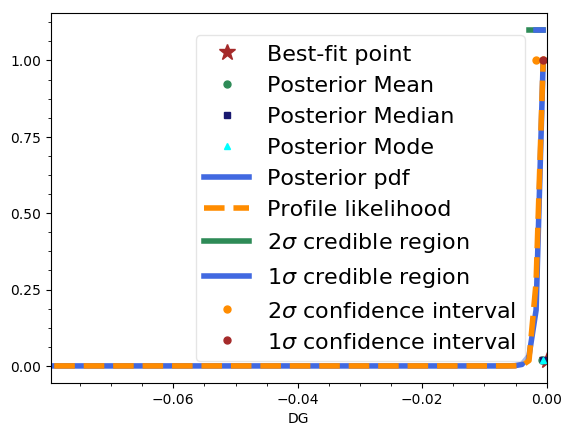
\includegraphics[width=0.49\textwidth]{figs/DG.png}
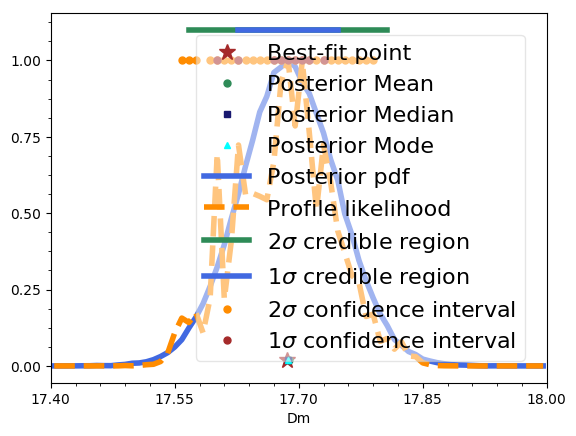
\includegraphics[width=0.49\textwidth]{figs/Dm.png}\\
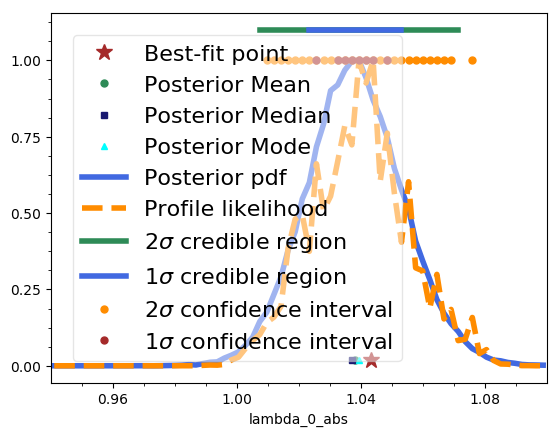
\includegraphics[width=0.49\textwidth]{figs/lambda_0_abs.png}
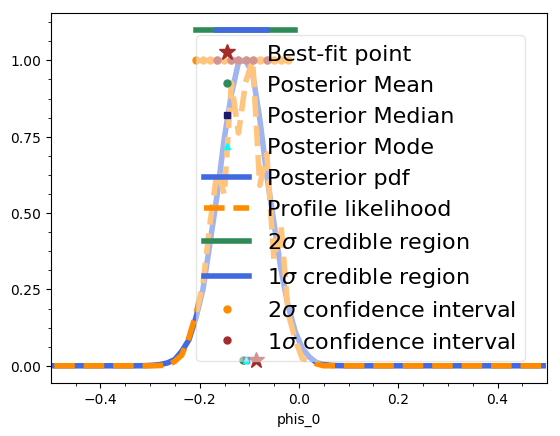
\includegraphics[width=0.49\textwidth]{figs/phis_0.png}\\
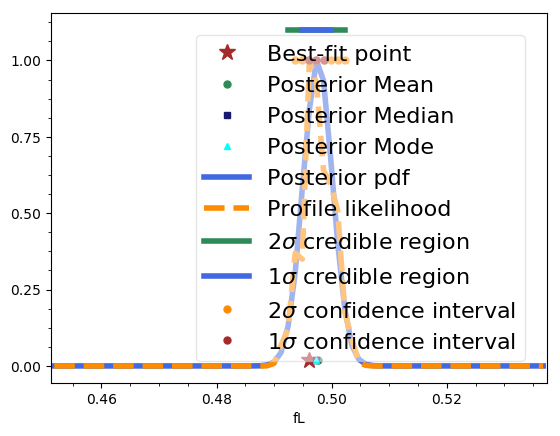
\includegraphics[width=0.49\textwidth]{figs/fL.png}
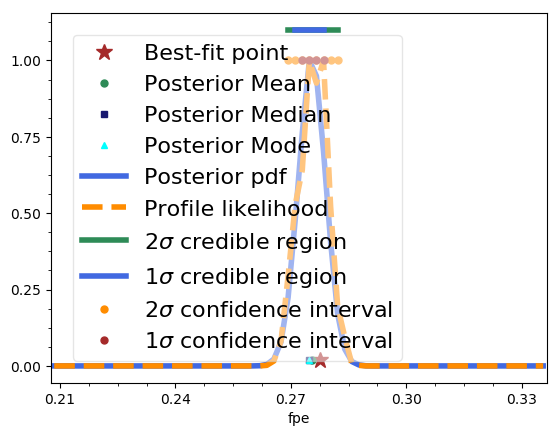
\includegraphics[width=0.49\textwidth]{figs/fpe.png}\\
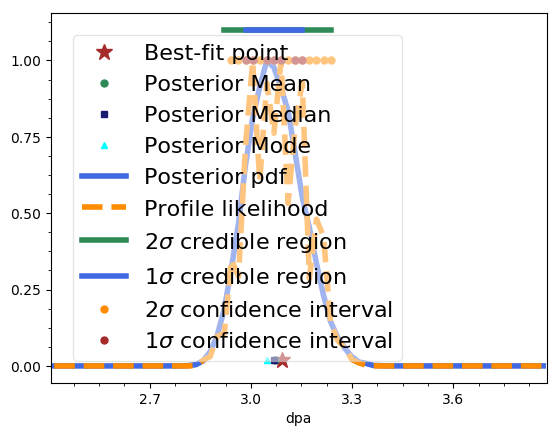
\includegraphics[width=0.49\textwidth]{figs/dpa.png}
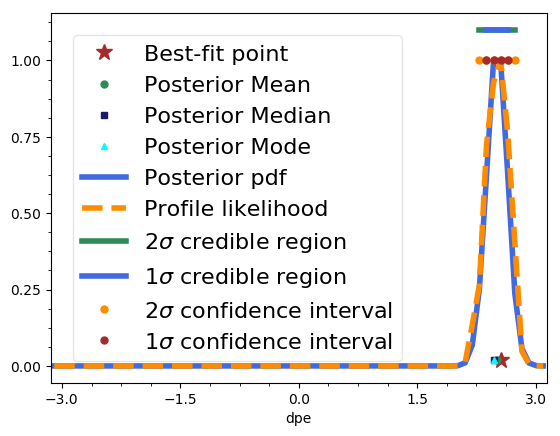
\includegraphics[width=0.49\textwidth]{figs/dpe.png}\\
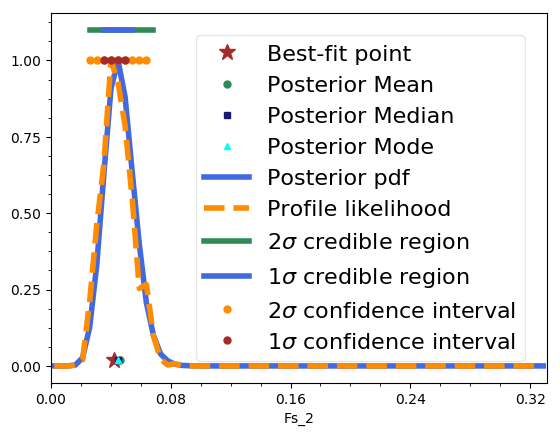
\includegraphics[width=0.49\textwidth]{figs/Fs_2.png}
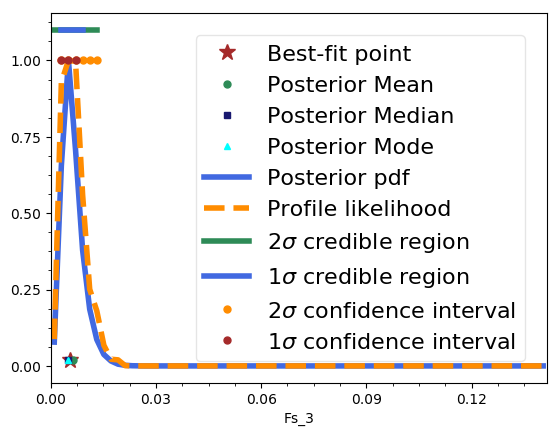
\includegraphics[width=0.49\textwidth]{figs/Fs_3.png}\\
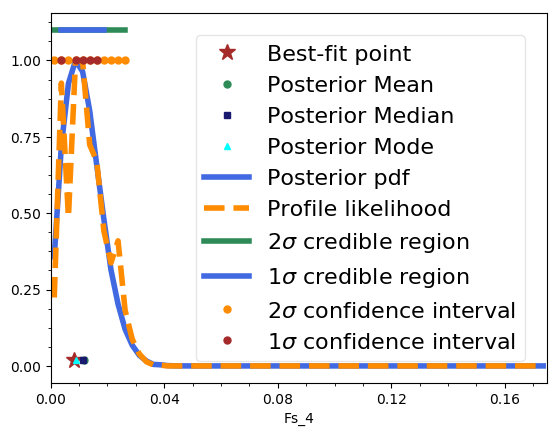
\includegraphics[width=0.49\textwidth]{figs/Fs_4.png}
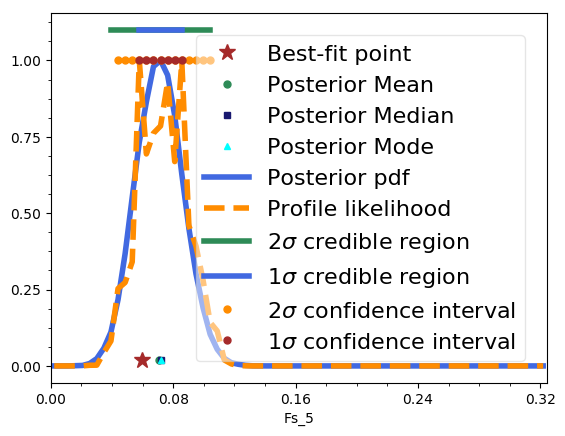
\includegraphics[width=0.49\textwidth]{figs/Fs_5.png}\\
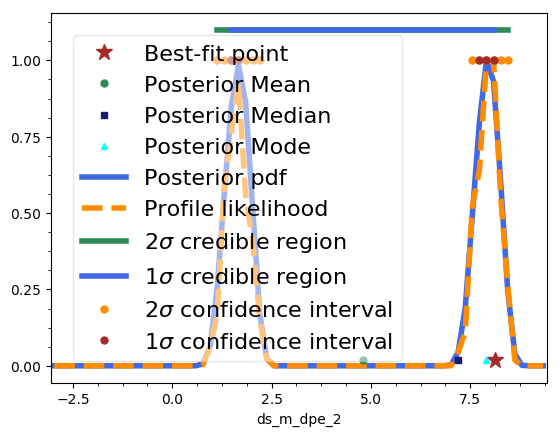
\includegraphics[width=0.49\textwidth]{figs/ds_m_dpe_2.png}
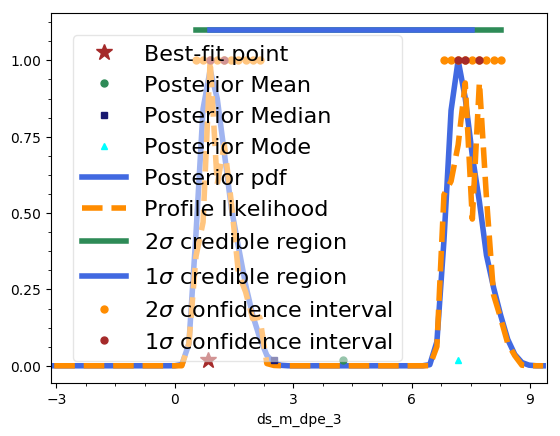
\includegraphics[width=0.49\textwidth]{figs/ds_m_dpe_3.png}\\
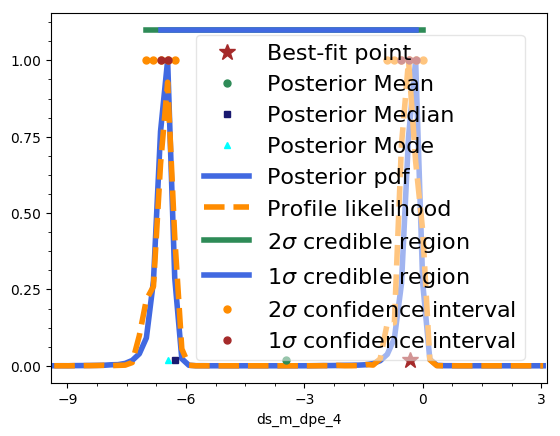
\includegraphics[width=0.49\textwidth]{figs/ds_m_dpe_4.png}
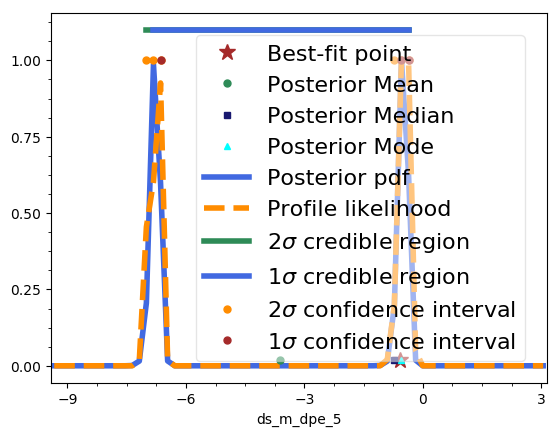
\includegraphics[width=0.49\textwidth]{figs/ds_m_dpe_5.png}\\
\label{fig:phisMN1D}
\end{center}

\begin{center}
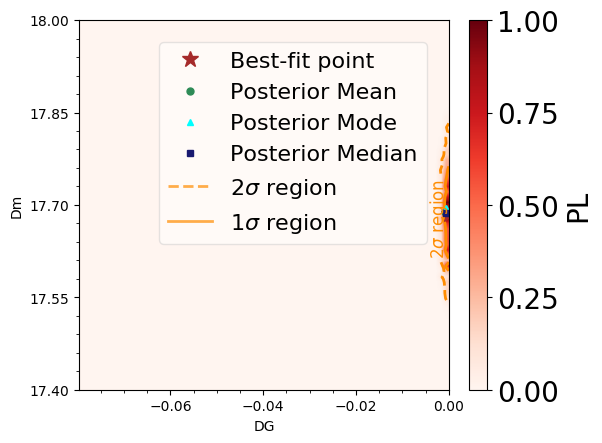
\includegraphics[width=0.49\textwidth]{figs/DG_vs_Dm.png}
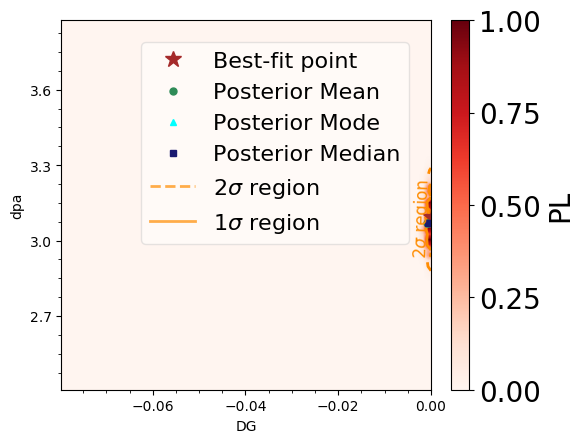
\includegraphics[width=0.49\textwidth]{figs/DG_vs_dpa.png}\\
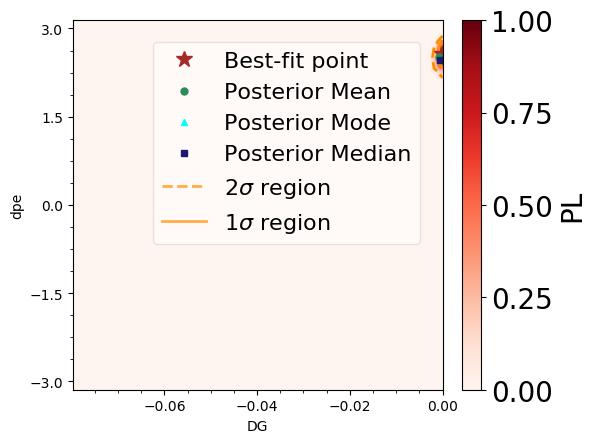
\includegraphics[width=0.49\textwidth]{figs/DG_vs_dpe.png}
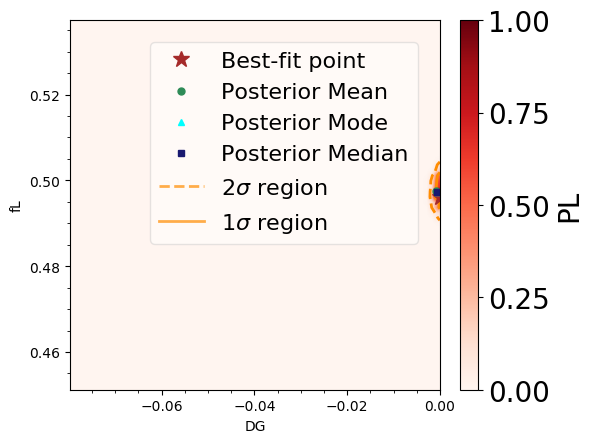
\includegraphics[width=0.49\textwidth]{figs/DG_vs_fL.png}\\
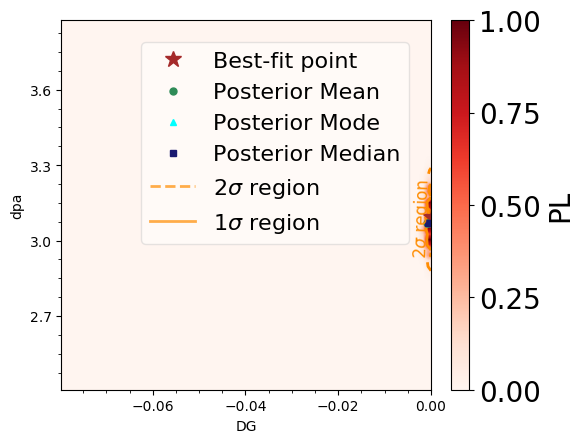
\includegraphics[width=0.49\textwidth]{figs/DG_vs_dpa.png}
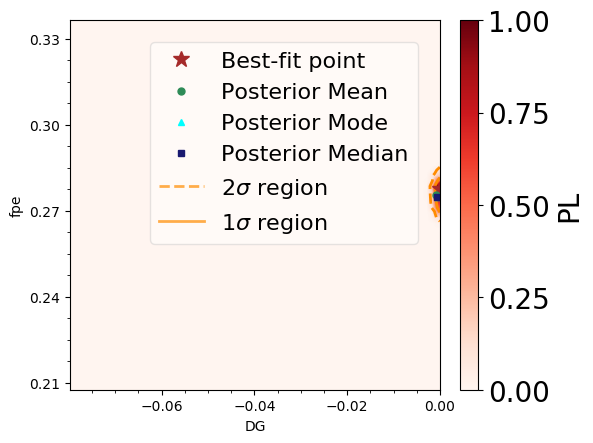
\includegraphics[width=0.49\textwidth]{figs/DG_vs_fpe.png}\\
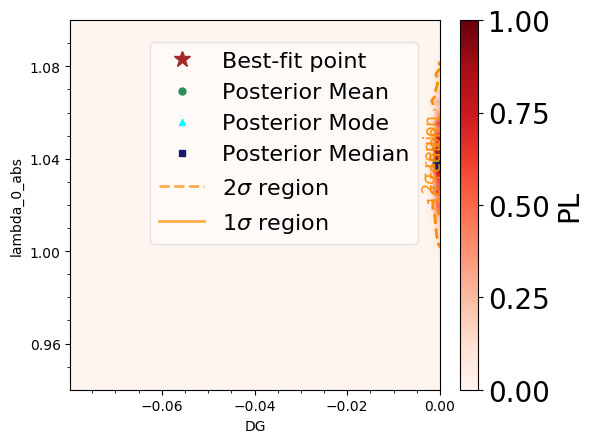
\includegraphics[width=0.49\textwidth]{figs/DG_vs_lambda_0_abs.png}
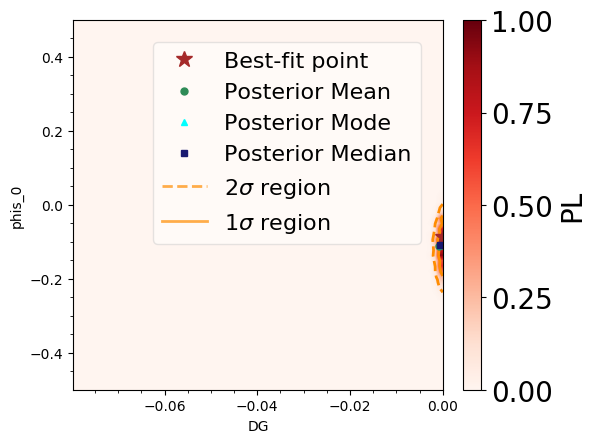
\includegraphics[width=0.49\textwidth]{figs/DG_vs_phis_0.png}\\
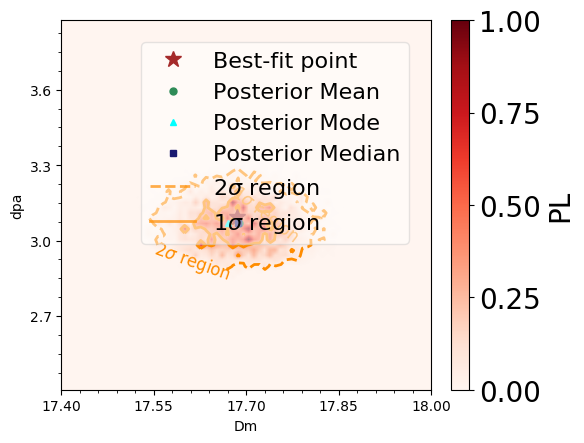
\includegraphics[width=0.49\textwidth]{figs/Dm_vs_dpa.png}
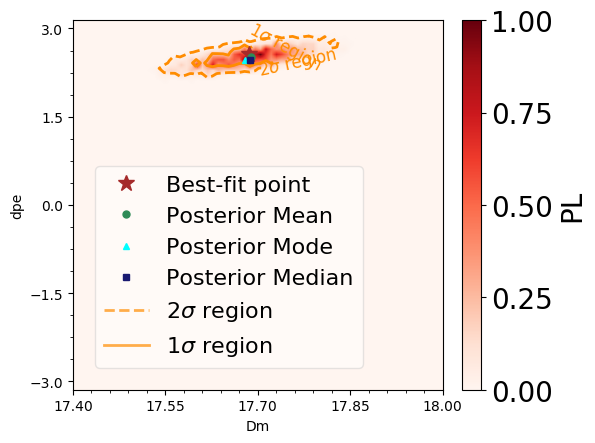
\includegraphics[width=0.49\textwidth]{figs/Dm_vs_dpe.png}\\
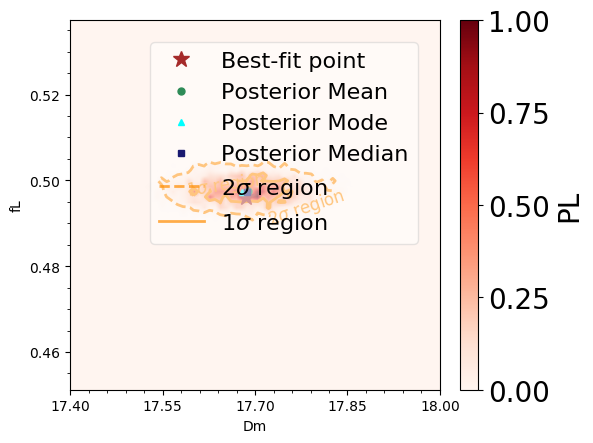
\includegraphics[width=0.49\textwidth]{figs/Dm_vs_fL.png}
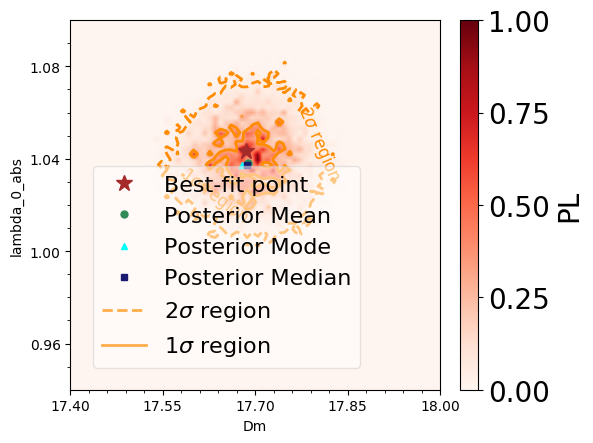
\includegraphics[width=0.49\textwidth]{figs/Dm_vs_lambda_0_abs.png}\\
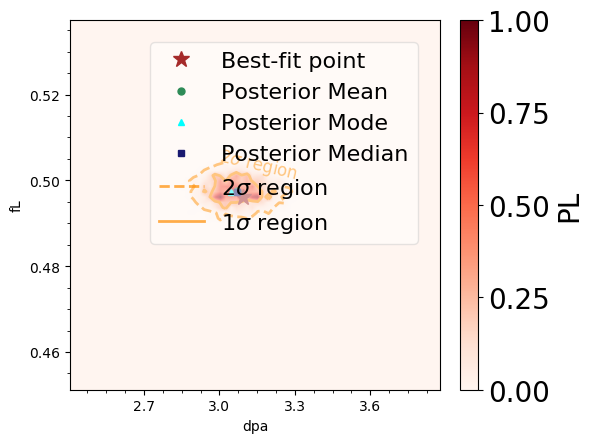
\includegraphics[width=0.49\textwidth]{figs/dpa_vs_fL.png}
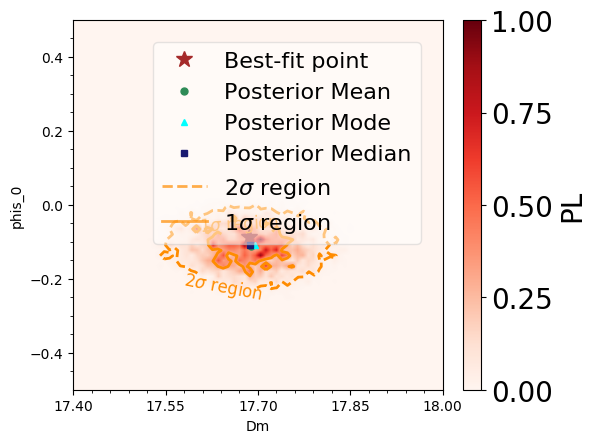
\includegraphics[width=0.49\textwidth]{figs/Dm_vs_phis_0.png}\\
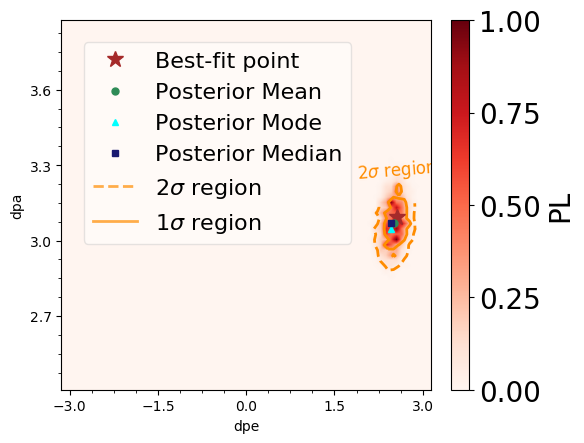
\includegraphics[width=0.49\textwidth]{figs/dpe_vs_dpa.png}
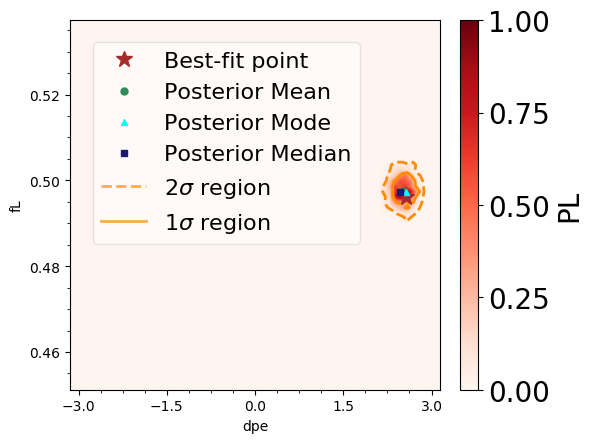
\includegraphics[width=0.49\textwidth]{figs/dpe_vs_fL.png}\\
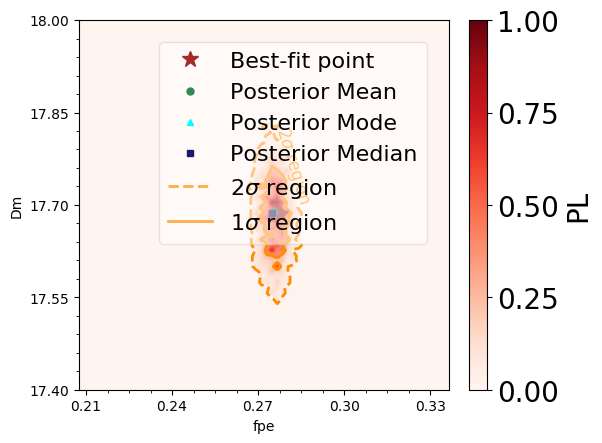
\includegraphics[width=0.49\textwidth]{figs/fpe_vs_Dm.png}
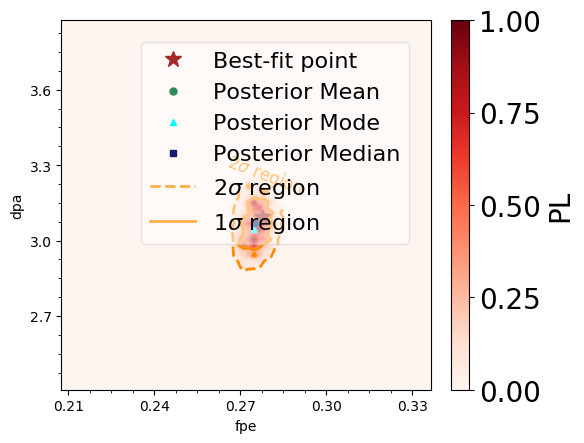
\includegraphics[width=0.49\textwidth]{figs/fpe_vs_dpa.png}\\
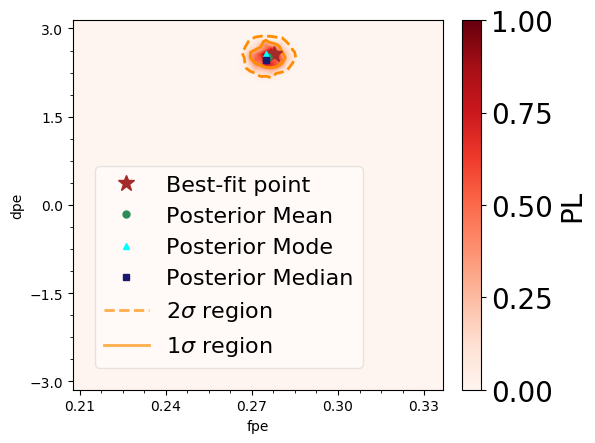
\includegraphics[width=0.49\textwidth]{figs/fpe_vs_dpe.png}
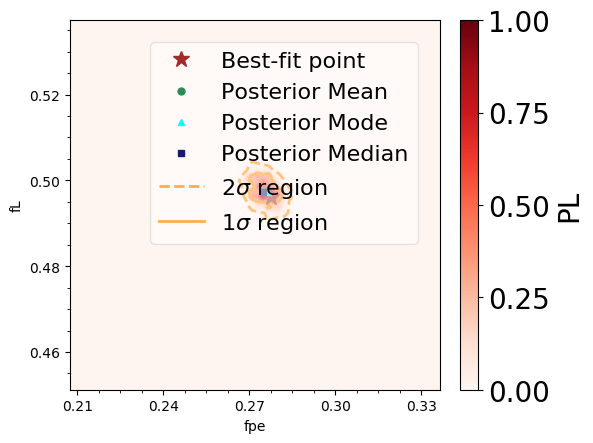
\includegraphics[width=0.49\textwidth]{figs/fpe_vs_fL.png}\\
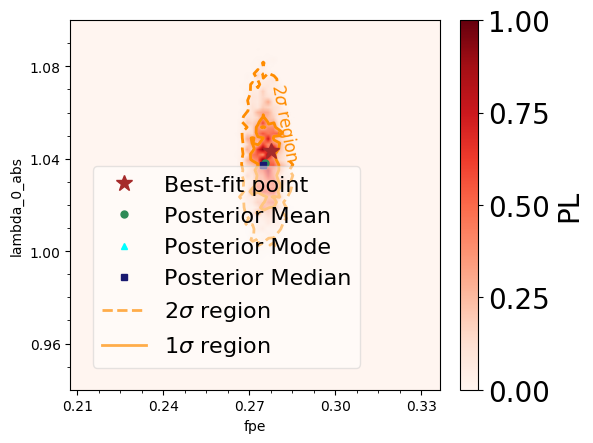
\includegraphics[width=0.49\textwidth]{figs/fpe_vs_lambda_0_abs.png}
\includegraphics[width=0.49\textwidth]{figs/fpe_vs_phis_0.png}\\
\includegraphics[width=0.49\textwidth]{figs/lambda_0_abs_vs_dpa.png}
\includegraphics[width=0.49\textwidth]{figs/lambda_0_abs_vs_dpe.png}\\
\includegraphics[width=0.49\textwidth]{figs/lambda_0_abs_vs_fL.png}
\includegraphics[width=0.49\textwidth]{figs/phis_0_vs_dpa.png}\\
\includegraphics[width=0.49\textwidth]{figs/phis_0_vs_dpe.png}
\includegraphics[width=0.49\textwidth]{figs/phis_0_vs_fL.png}\\
\includegraphics[width=0.49\textwidth]{figs/phis_0_vs_lambda_0_abs.png}
\label{fig:phisMN2D}
\end{center}

%%%%%%%%%%%%%%%%%
%%%%%%%%%%%%%%%%%%%%%%%%%%%%%%%%%%%%%%%%%%%%%%%%%%%%%%%%%%%%%%%%%%%%%%%%%%%%%%%%%%
%%%%%%%%%%%%%%%%%%%%%%%%%%%%%%%%%%%%%%%%%%%%%%%%%%%%%%%%%%%%%%%%%%%%%%%%%%%%%%%%%%

\red{
\begin{enumerate}
\item Description of the tool
\item Description of the plots + Methodology
\item Conclusions from the plots 
\end{enumerate}
}

\subsection{\texttt{MultiNest}}
\ref{sec:MultiNest}
\texttt{MultiNest} is a multimodal, parallelizable nested sampling algorithm. 

It calculates the evidence, with an associated error estimate, and produces posterior samples from distributions that may contain multiple modes and/or pronounced (curving) degeneracies in high dimensions. The algoritm also naturally identifies individual modes of a distribution, allowing for the evaluation of the 'local' evidence and parameter constraints associated with each mode separately.
%%It outperforms \red{in efficiency and robustness} the existing Markov chain Monte Carlo (MCMC) sampling, used for parameter estimation. This can be computationally intensive, and often experience problems in sampling efficiently from a multimodal posterior distribution or one with large (curving) degeneracies between parameters, particularly in high dimensions. Besides, MCMC methods often require careful tuning of the proposal distribution, and testing for convergence can be problematic. %%% The existing preferred evidence evaluation method, again based on MCMC techniques, is thermodynamic integration (greater computational expense to compute the key ingredient, the Bayesian evidence)
%% Bayesian evidence = marginalized likelihood = marginal density of the data

%%Nested sampling is a MC method targetted at the efficient calculation of the evidence, also producing posterior inference as a by-product. Their algorithm uses an elliptical bound containing the current point set at each stage of the process to restrict the region around the posterior peak from which new samples are drawn. 
%%Highly inefficient for multimodal posteriors, the notion of clustered nested sampling is introduced. 
\subsubsection{Bayesian inference}
Bayesian inference provides a consistent approach to the estimation of a set of parameters $\Theta$ in a model or hypothesis H, for the data, D, $Pr(\Theta|D,H)$, according to Bayes' theorem \red{ref}. 
The Bayesian evidence, $Pr(D|H) \equiv \mathcal{Z}$, usually ignored in parameter estimation problems, plays a central role in model selection. It is the factor required to normalize the posterior over $\Theta$. 
\begin{equation}
\mathcal{Z} = \int \mathcal{L}(\Theta) \pi(\Theta)d^D\Theta
\end{equation}
Where D is the dimensionality of the parameter space. The evaluation of this integral is a challenging numerical task. %%

\subsubsection{Nested sampling}
Nested sampling is a MC technique aimed at efficient evaluation of the Bayesian evidence, but also produces posterior inferences as a by-product. 
It exploits the relation between the likelihood and prior volumeeta ($dX = \pi(\Theta)d^D\Theta$) to transform the multidimensional evidence integral into a one-dimensional integral:
\begin{equation}
\mathcal{Z} = \int_0^1 \mathcal{L}(X) dX
\end{equation}
$\mathcal{L}(X)$ is a monotically decreasing function of X. Thus:
\begin{equation}
\mathcal{Z} = \sum_{i=1}^M \mathcal{L}_i w_i dX
\end{equation}

\begin{itemize}
\item i=0 and N 'active' or 'live' samples are drawn from the full prior $\pi(\Theta)$, so that the initial prior volume is $X_0 = 1$.
\item Samples are sorted in order of their likelihood and the smallest ($\mathcal{L}_0$) is discarded, becoming 'inactive', and replaced by a point drawn from the prior subject to the constraint $\mathcal{L} > \mathcal{L}_0$. $X_1 = t_1 X_0, \ Pr(t) = Nt^{N-1}$
\item Repeat previous tep, until the entire prior volume has been traversed. The algorithm thus travels through nested shells of likelihood as the prior volume is reduced. 
\item $X_i = \exp{(-i/N)}$
\item Algorithm is terminated on determining the evidence to some specified precision:
$\Delta \mathcal{Z} = \sum_{i=1}^N \mathcal{L}_j w_{M+j}, \ w_{M+j} = X_M / N$
where N are the active points. 
\end{itemize}
Once the evidence is found, posterior inferences can be easily generated using inactive and active points generated in the nested sampling process. Each point is assigned the weight:
\begin{equation}
p_j = \frac{\mathcal{L}_j w_j}{\mathcal{Z}}
\end{equation}

\subsubsection{Ellipsoidal nested sampling}
The most chalenging task in implementing the nested sampling algorithm is drawing samples from the prior within the hard constraint $\mathcal{L} > \mathcal{L}_i$ at each iteration \textit{i}. 
Ellipsoidal nested sample tries to overcome this problem by approximating the iso-likelihood contour $\mathcal{L} = \mathcal{L}_i$ by a D-dimensional ellipsoid, determined from the covariance matrix of the current set of active points. New points are selected from the prior within this ellipsoidal bound until one fulfills the aforementioned conditioned. 
This method is not well suited to multimodal distribution. Its efficiency is improved by identifying distinct \textit{clusters} of active points that are well separated and constructing an individual (enlarged) ellipsoid bound for each cluster. 

\subsubsection{The \texttt{MultiNest} algorithm}
The clusters in which the set of active points are partitioned are then enclosed in ellipsoids and a new point is drawn from the set of these 'overlapping' ellipsoids (properly taking into account the overlaps. For highly multimodal problems, the nested sampling algorithm would require a large number of active points to ensure that all the modes are detected, resulting in a slow convergence.  

\begin{comment}
Partitioning the set of active points into as many sub-clusters as possible to allow maximum flexibility in following the degeneracy. Using a new algorithm.  
These clusters are then enclosed in ellipsoids and a new point is drawn from the set of these 'overlapping' ellipsoids, correctly taking into account the overlaps. 
The algorithm requires the points to be uniformly distributed in the parameter space. If the prior is uniform, this condition is already satisfied. Otherwise, the construction of a D-dimensional unit hypercube is needed. 
It is possible that the ellipsoids found by the Algorithm don't enclose the entire iso-likelihood contour, since the ellipsoidal approximation to a region in the prior space might not be perfect. This can be accounted for using X/e as the desired minimum volume, where 1/e is an \textit{enlargement factor}. 
For highly multimodal problems, the nested sampling algorithm would require a large number of active points to ensure that all the modes are detected, resulting in a slow convergence. 
Nested sampling does not require the number of active points to remain constant, provided the fraction by which the prior volume is decreased after each iteraction is adjusted accordingly. Without knowing anything about the posterior, we can use the largest evidence contribution that can be made by the remaining portion of the posterior at the $i^{\rm th}$ iteration $\Delta\mathcal{Z}_i = \mathcal{L}_{\rm max}X_i$ as the guide in reducing the number of acctive points by assuming that the change in $\Delta\mathcal{Z}$ is linear locally. The number of active points $N_i$ at the $i^{th}$ iteration is:
\begin{equation}
N_i = N_{i-1} - N_{min}\frac{\Delta\mathcal{Z}_{i-1} - \Delta\mathcal{Z}_i}{\Delta\mathcal{Z} - \rm tol}
\end{equation}
where $N_{min}$ is the minimum number of active points allowed and tol is the tolerance on the final evidence used in the stopping criterion. 
\end{comment}

The \texttt{MultiNest} algorithm is controlled by two parameters:
\begin{itemize}
\item The number of active points, N. It should be large enough that, in the initial sampling from the full prior space, there is a high probability that at least one point lies in the 'basin of attraction' of each mode of the posterior. Also sufficiently large so that all the regions of the parameter space are sampled adequately, bigger than the dimensionality of the parameter space. 
\item The maximum efficiency, \textit{e}, that controls the sampling volume at each iteration, which is eual to the sum of the volumes of the ellipsoids enclosing the active point set. 
\end{itemize}
